\section{Analysis}

%Analysis may involve: Interpretation, Presentation, comparison and confirmation

% The analysis chapter will present and discuss the main findings and outcomes, with limits being acknowledged (ie. Survey response levels, generalisability of results, reliability of tests, factos outwith your control.)

\subsection{Data analysis}

% Outline key variables and hypostheses being tested. 
The shortest path length distribution, degree correlation coefficient and degree correlation matrices will be used to compare each topology in a given set. 
Side by side visual comparison between the simulated network topology and the measured network topology will also be presented. 

This data is numerical and discrete, each topologies results using these metrics will be evaluated and compared with the aim of establishing the characteristics which define real-world topologies, and also if randomly generated topologies can successfully emulate these characteristics. The data will be collected through the use of functions from the NetworkX python library, to evaluate graph objects represented through GML files. 

\begin{figure}
    \centering
    \verb|nx.degree_assortativity_coefficient(G)| \verb|nx.all_pairs_shortest_path_length(G)|
    \caption{Functions used to evaluate topolgies}
    \label{fig:enter-label}
\end{figure}

% Data preparation
The 

% Tools/Mathimatical models used for analysis
Experimental data will be directly plotted using matplotlib, a python library, "Matplotlib is a comprehensive library for creating static, animated, and interactive visualizations in Python"\cite{matplotlib},  from which it can be easily processed. The mean, mode, median and standard deviation will be presented for each finding. Analysis of the implemented model will be carried out using several metrics in order to illustrate comparisons between it's performance and the original model's performance. Several plot types such as scatter plots, line plots and violin plots will be used to visualize; negative and positive correlations and also to represent the standard deviation of results respectively. Furthermore, tables of data will also be used to provide accurate numerical data in a straightforward manner.

% 6. Connect methods to research objectives

%focusing on the study, hypothesis, sample groups you wish to address, and the limitations you have faced.

\subsection{Results}


\subsubsection{Topology set 1}
As shown from the comparison between the shortest path length distribution of Erdos-Renyi, Barabasi-Albert, and real-world topologies, Dataxchange and Layer42; the Erods-Renyi graph with p=0.5 has most closely matches the distribution of shortest path lengths to the real-world topology Dataxchange. With both topologies having frequencies of approximately 0.5 and 0.6 of shortest path length 1.0 respectively. However, there is still some disparity between the frequency of higher shortest path length values between the two topologies. Additionally, the Erdos-Renyi graph with p=0.5 also most closely matches the Layer42 network, with the difference between the shortest path length value 1.0 being approximately 1 and approximately 0.75 for shortest path length value 2.0.  

\begin{figure}
    \centering
    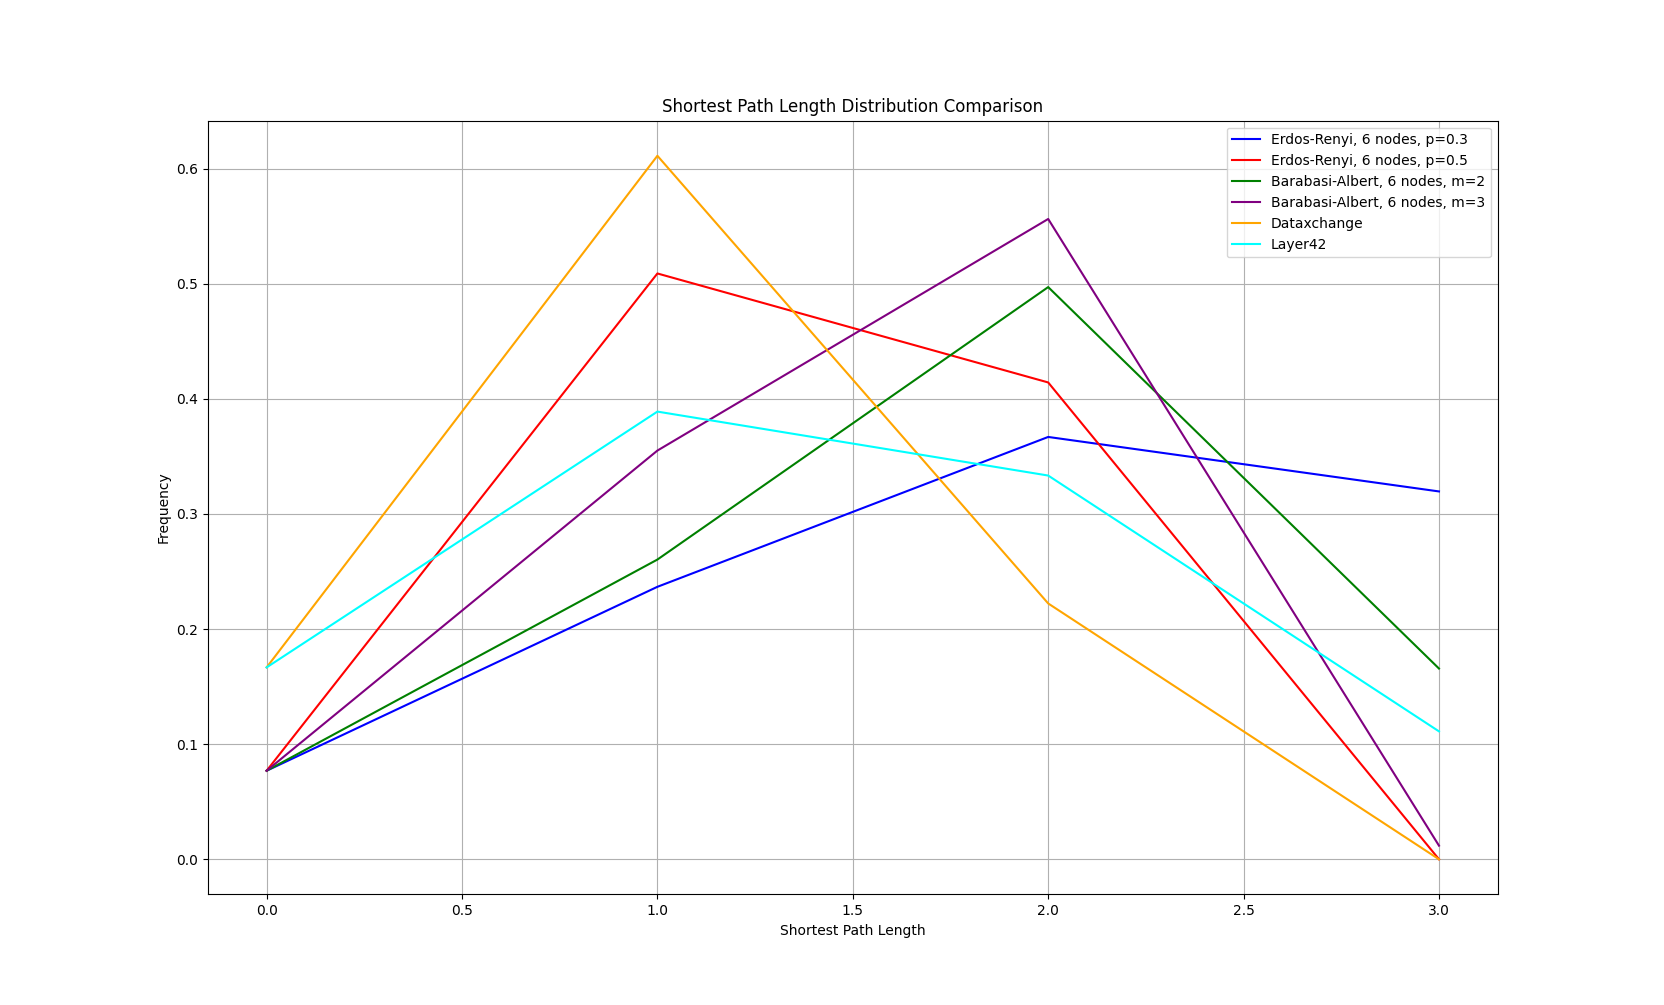
\includegraphics[width=0.9\linewidth]{images/FINAL-TOPO-COMP/line-6.png}
    \caption{Shortest path length distribution comparison, set 1}
    \label{fig:enter-label}
\end{figure}

\begin{figure}
    \centering
    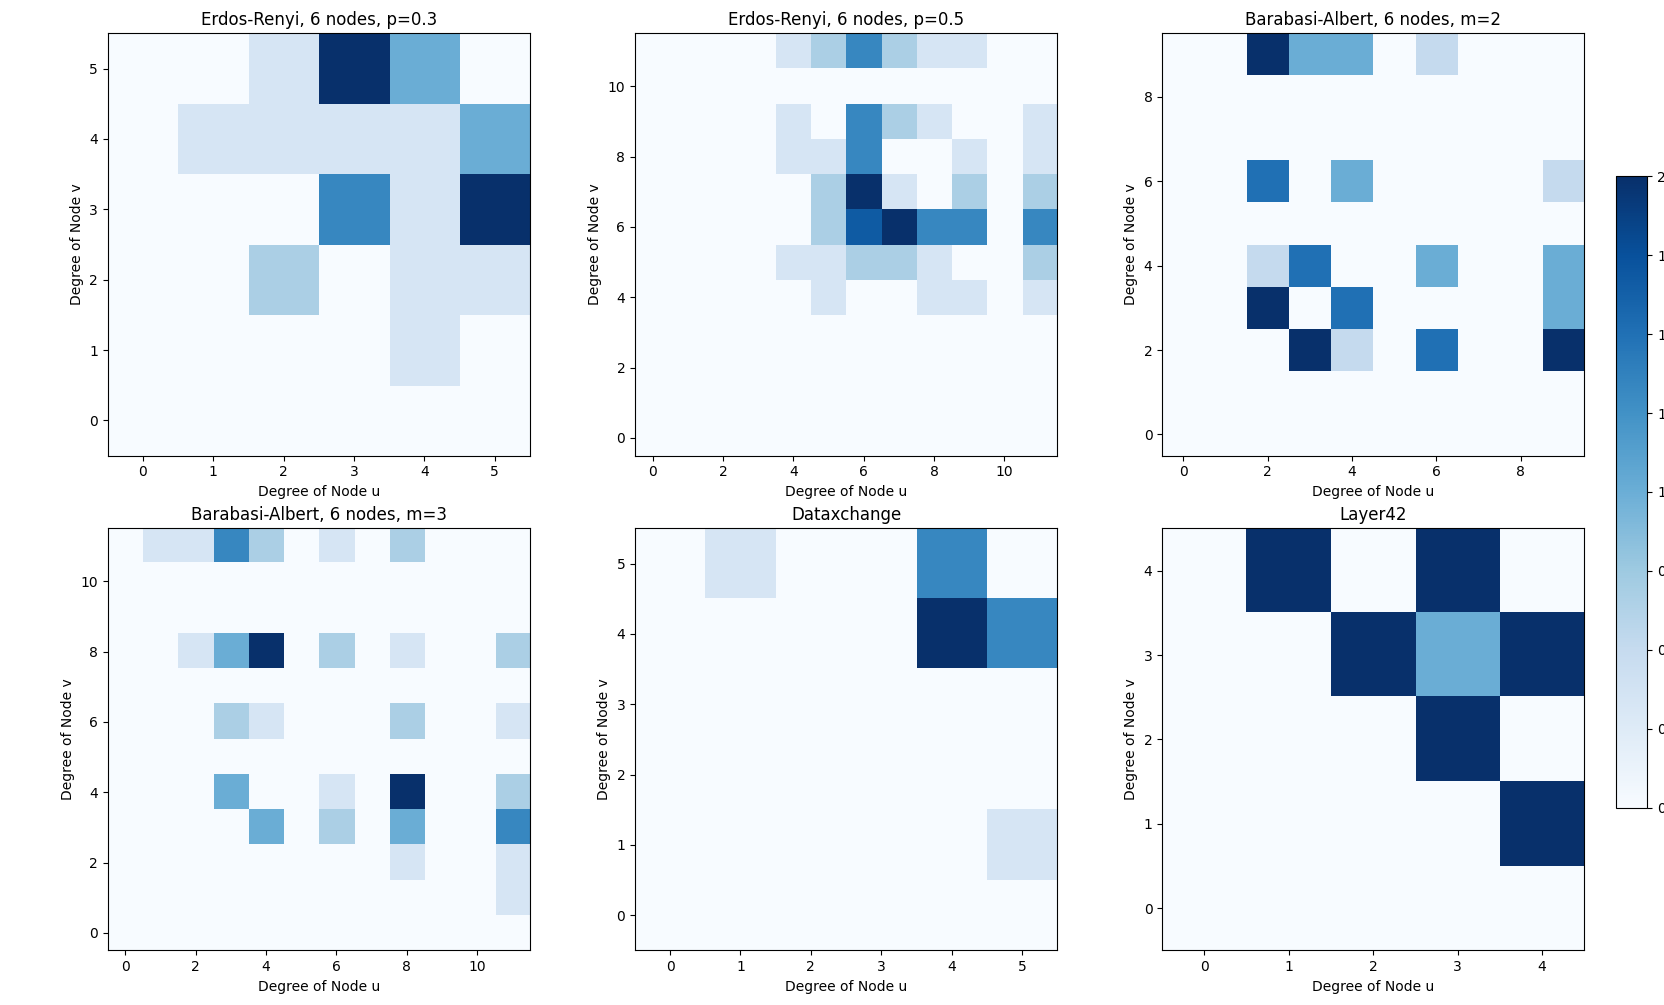
\includegraphics[width=0.9\linewidth]{images/FINAL-TOPO-COMP/Degree-correlation-matrices/6-matrix.png}
    \caption{Degree correlation matrix, set 1}
    \label{fig:enter-label}
\end{figure}

However, when taking into consideration the degree correlation coefficient, the Barabasi-Albert graph with m=3, is the most closely correlated to both the Dataxchange and Layer42 networks. The Barabasi-Albert generated network has an $r$ value of -0.49, compared with $r$ values of -0.45 and -0.6 for Dataxchange and Layer42 respectively.  

\begin{figure}
    \centering
    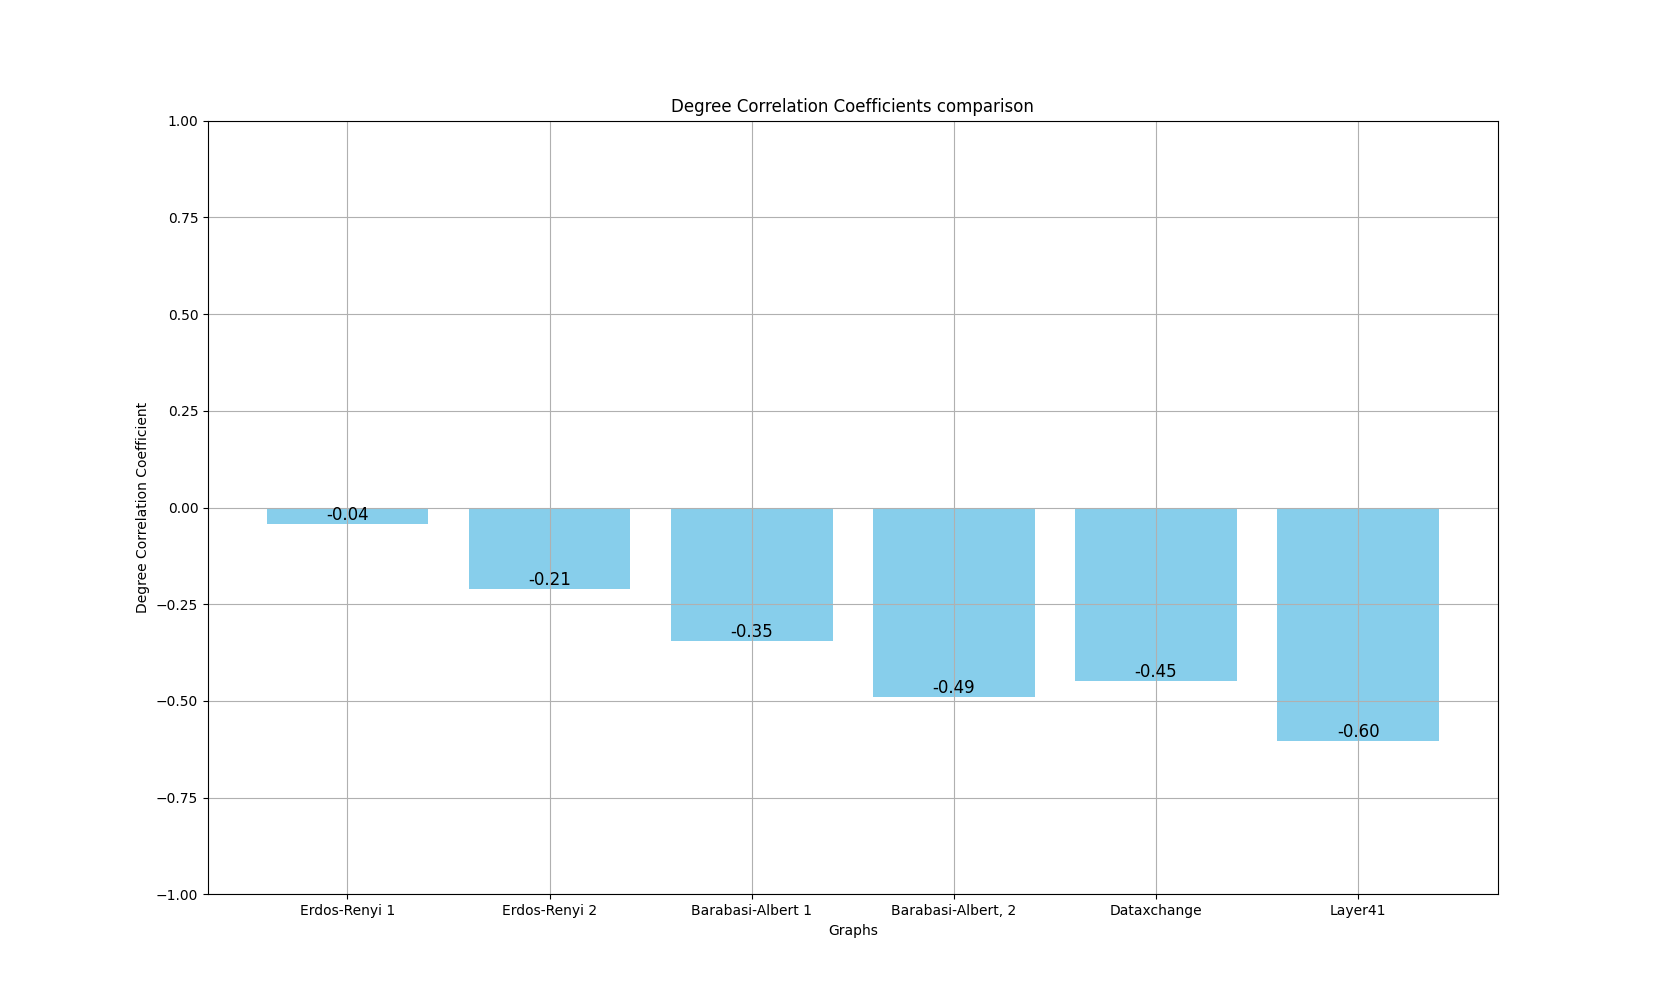
\includegraphics[width=0.9\linewidth]{images/FINAL-TOPO-COMP/Degree-correlation-coeff/deg-coeff-6.png}
    \caption{Degree correlation coefficient, set 1}
    \label{fig:enter-label}
\end{figure}

\subsubsection{Topology set 2}
Similarly to the previous topology set, the Erdos-Renyi graph generated using $p=0.3$, most closely matches both the Navigata and Nsfnet topologies with regards to shortest path length distribution. Particularly so with the Navigata topology.

\begin{figure}
    \centering
    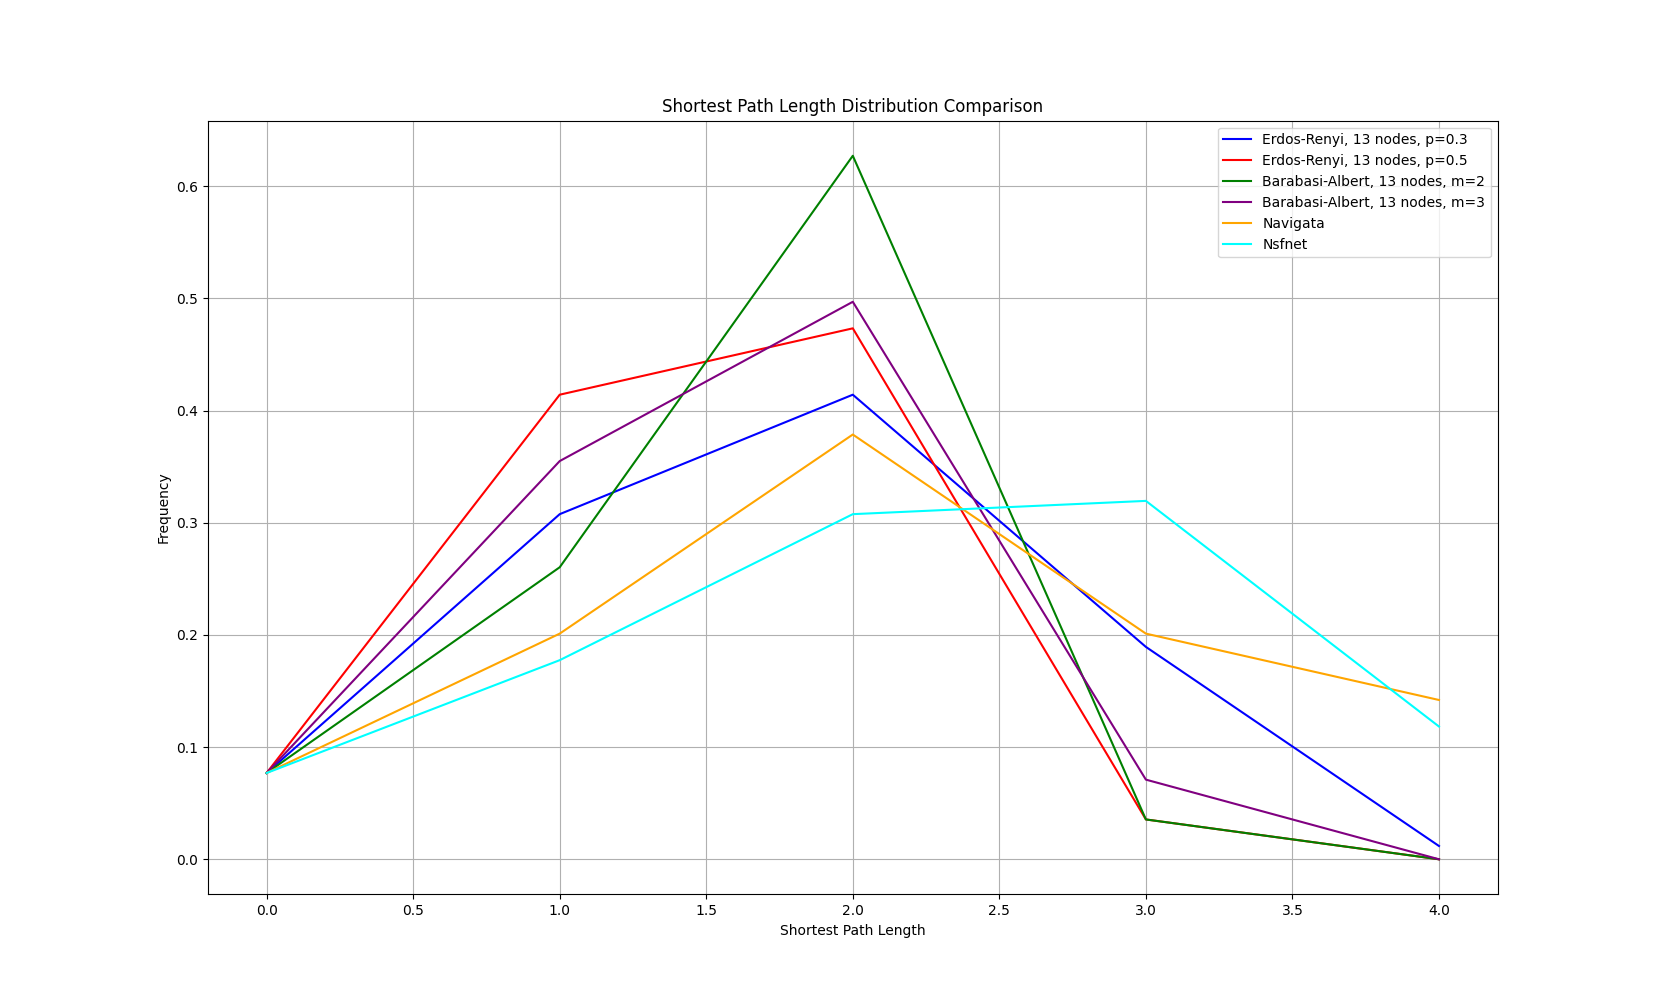
\includegraphics[width=0.9\linewidth]{images/FINAL-TOPO-COMP/line-13.png}
    \caption{Shortest path length distribution comparison, set 2}
    \label{fig:enter-label}
\end{figure}

\begin{figure}
    \centering
    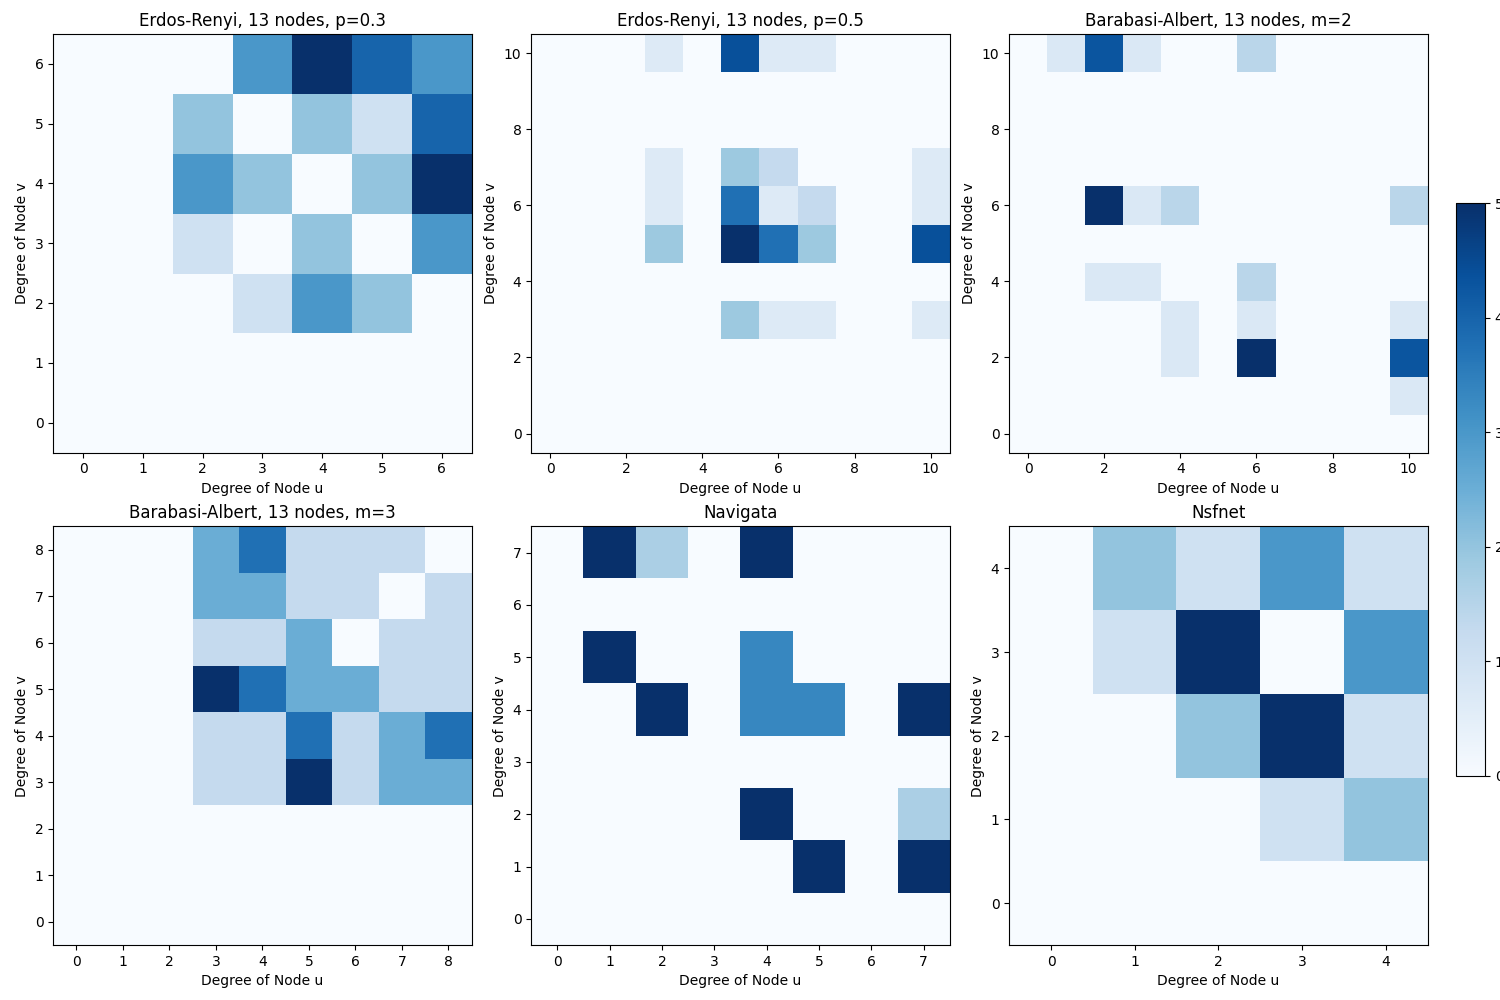
\includegraphics[width=0.9\linewidth]{images/FINAL-TOPO-COMP/Degree-correlation-matrices/13-matrix.png}
    \caption{Degree correlation matrix, set 2}
    \label{fig:enter-label}
\end{figure}

\begin{figure}
    \centering
    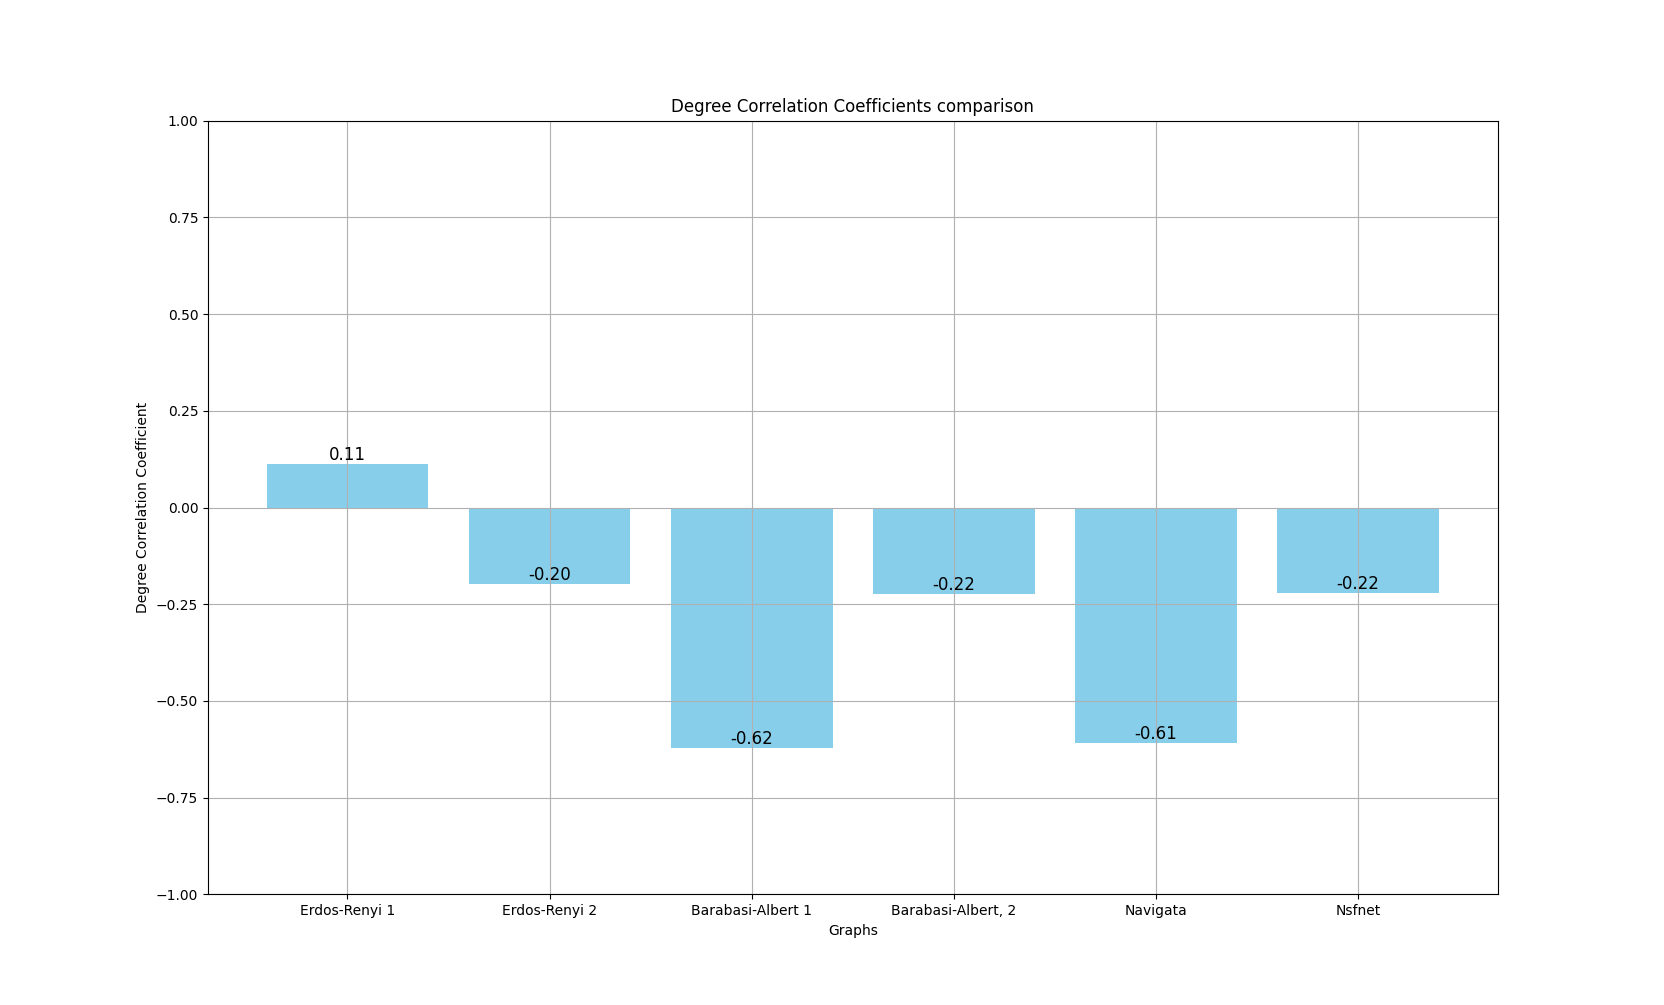
\includegraphics[width=0.9\linewidth]{images/FINAL-TOPO-COMP/Degree-correlation-coeff/deg-coeff-13.png}
    \caption{Degree correlation coefficient, set 2}
    \label{fig:enter-label}
\end{figure}

When comparing the degree correlation coefficient, both topologies generated using the Barabasi-Albert model match each of the real-world topologies respectively. With the m=2 model having a Degree correlation coefficent of -0.62, compared with Navigatas degree correlation coefficient of -0.61. Furthermore, the m=3 model has a degree correlation coefficient of -0.22 which is equal to Nsfnet's -0.22, additionally the Erdos-Renyi p=0.5 model is also close to Nsfnet with a degree correlation of -0.2. The Erdos-Renyi p=0.3 model has a positive degree correlation coefficient of 0.11, which categorises it as Dissasortative, the rest of the topologies have negative degree correlation coefficients categorising them as Assortative.

\subsubsection{Topology set 3}
None of the generated model's of size 20 nodes have a comparable Shortest path length distribution to either of the real-world models. The real-world topologies both have flatter shortest path length distribution profiles, peaking at approximately 0.3 frequency of a shortest path length 3. Contrastingly, the p=0.5 Erdos-Renyi generated topology rises sharply from 0 to peak at approximately 0.5 frequency for shortest path lengths 1 and 2, then sharply dropping back down to 0. Interestingly, the m=3 Barabasi-Albert model and p=0.3 Erdos-Renyi model have very similar Distribution profiles, peaking at approximately 0.6 frequency for a shortest path length of 2. 

\begin{figure}
    \centering
    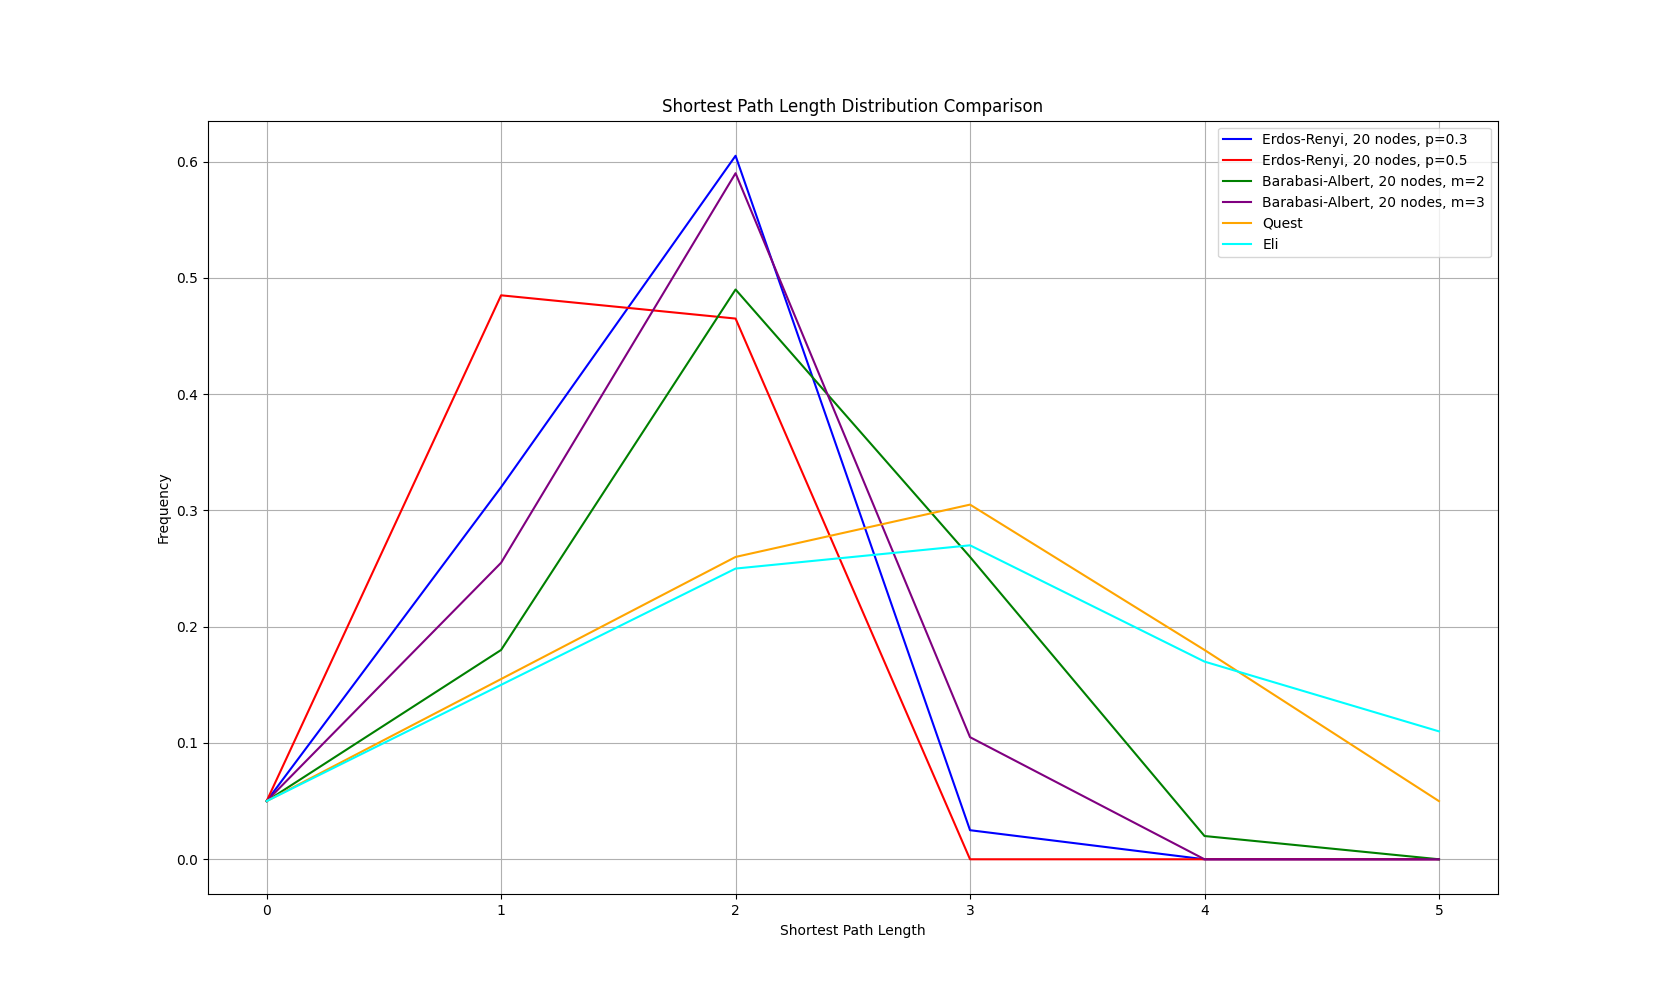
\includegraphics[width=0.9\linewidth]{images/FINAL-TOPO-COMP/line-20.png}
    \caption{Shortest path length distribution comparison, set 3}
    \label{fig:enter-label}
\end{figure}

\begin{figure}
    \centering
    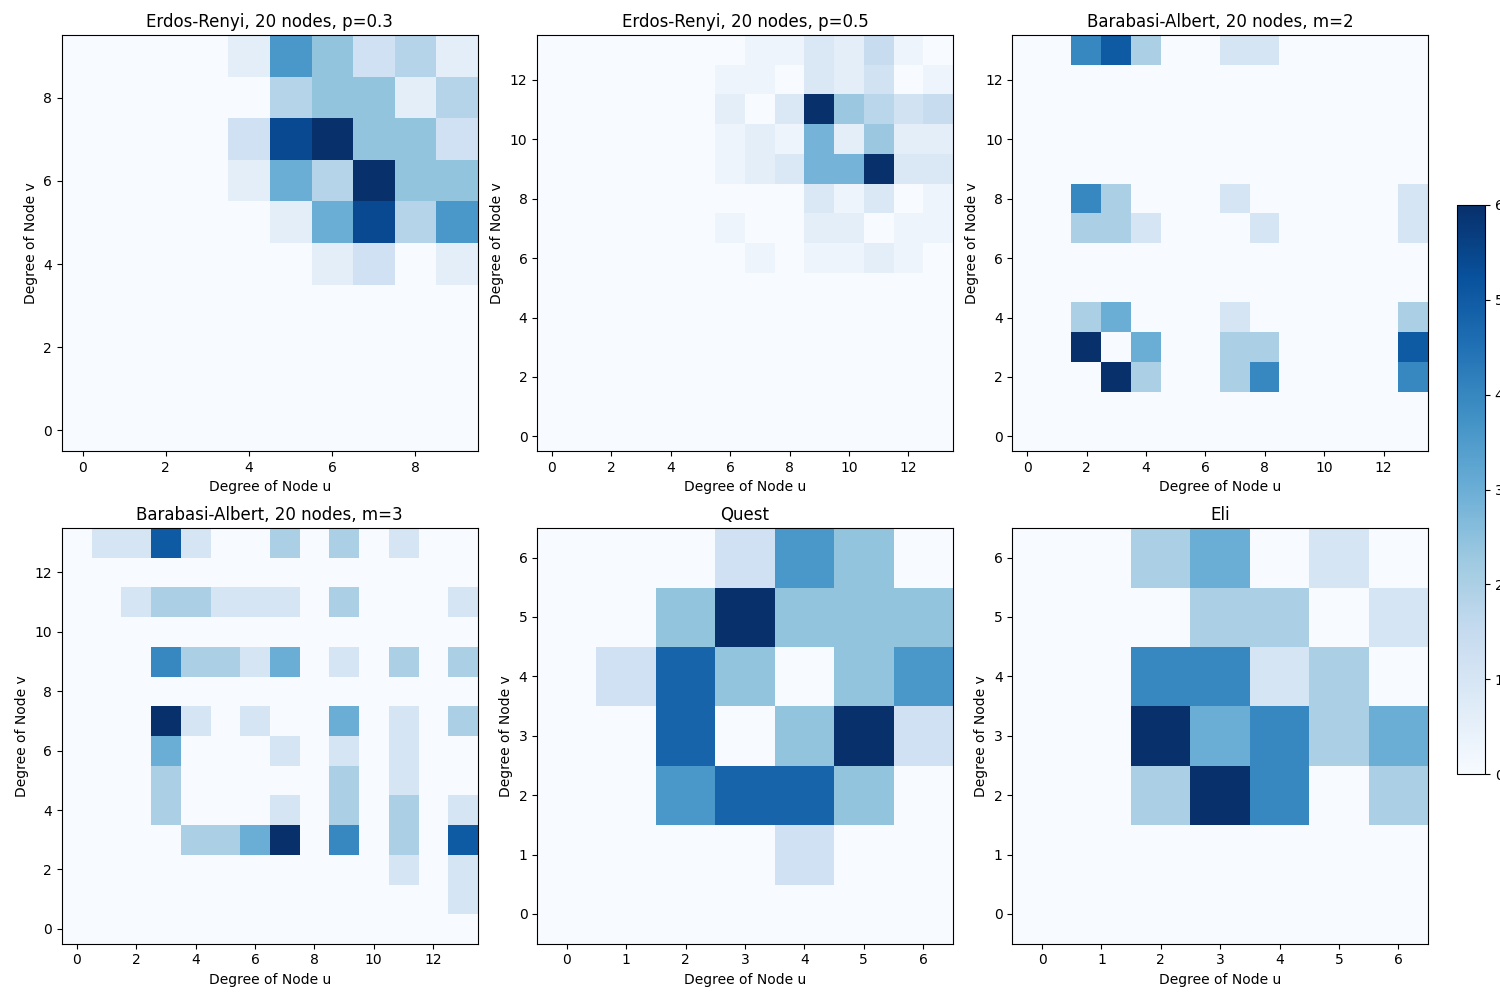
\includegraphics[width=0.9\linewidth]{images/FINAL-TOPO-COMP/Degree-correlation-matrices/20-matrix.png}
    \caption{Degree correlation matrix, set 3}
    \label{fig:enter-label}
\end{figure}

\begin{figure}
    \centering
    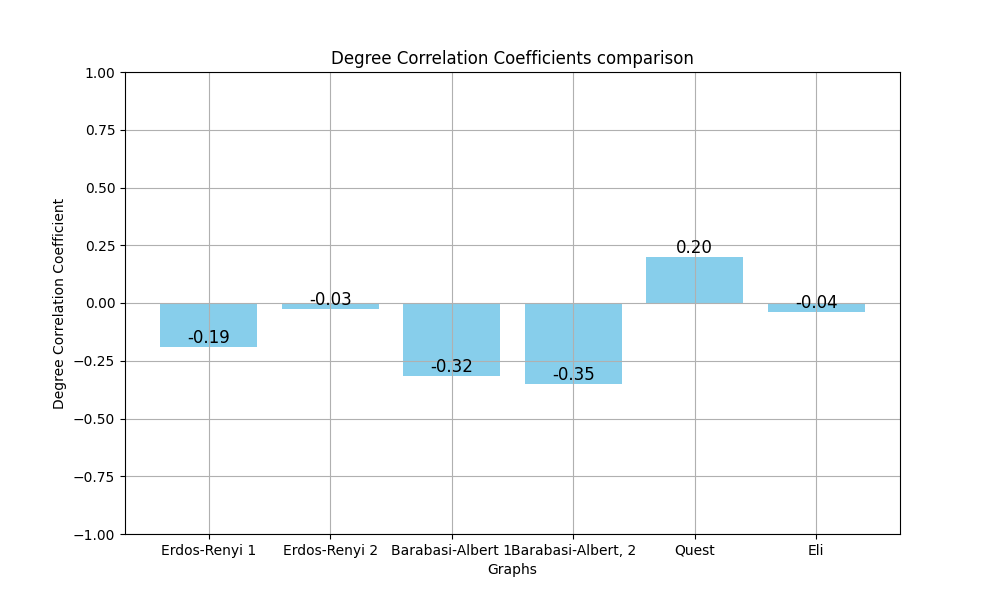
\includegraphics[width=0.9\linewidth]{images/FINAL-TOPO-COMP/Degree-correlation-coeff/deg-coeff-20.png}
    \caption{Degree correlation coefficient, set 3}
    \label{fig:enter-label}
\end{figure}
Through initial analysis of the varying degree correlation coefficients it is clear that the selected real-world topologies are distinct. With Quest having a positive degree correlation coefficient of 0.2 and Eli -0.04, this indicates that they are dissasortative and neutral topologies respectively. Out of the generated topologies the Erdos-Renyi p=0.5 model is similar to Eli, with a degree correlation coefficient of -0.03. 

\subsubsection{Topology set 4}
The shortest path length distribution of York, a real-world topology is relatively linear, maintaining a frequency of 0.3 shortest path lengths between 2 and 9. The generated topologies and Aconet have distinctly different profiles, with the Barabasi-Albert m=2 model having the closest shortest path length distribution to Aconet. Similarly to the previous topology set, the Erdos-Renyi p=0.3 and Barabasi-Albert m=3 model have very similar distributions, with both peaking just below 0.6 frequency for a shortest path length of 2. 

\begin{figure}
    \centering
    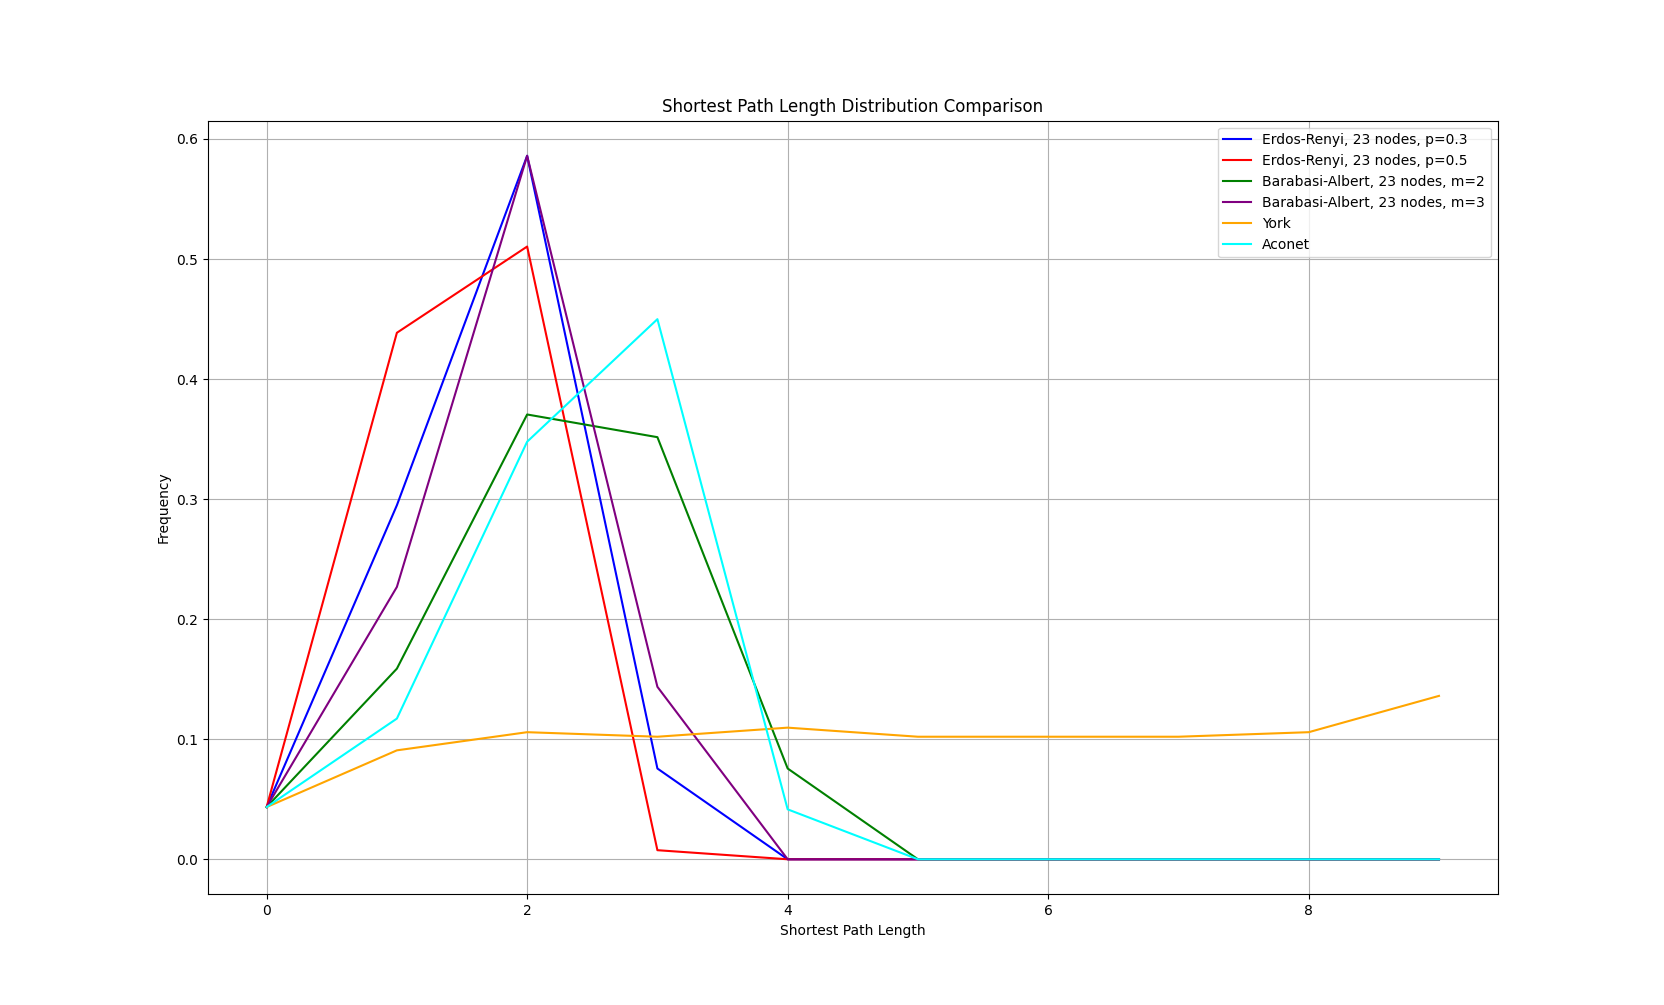
\includegraphics[width=0.9\linewidth]{images/FINAL-TOPO-COMP/line-23.png}
    \caption{Shortest path length distribution comparison, set 4}
    \label{fig:enter-label}
\end{figure}

\begin{figure}
    \centering
    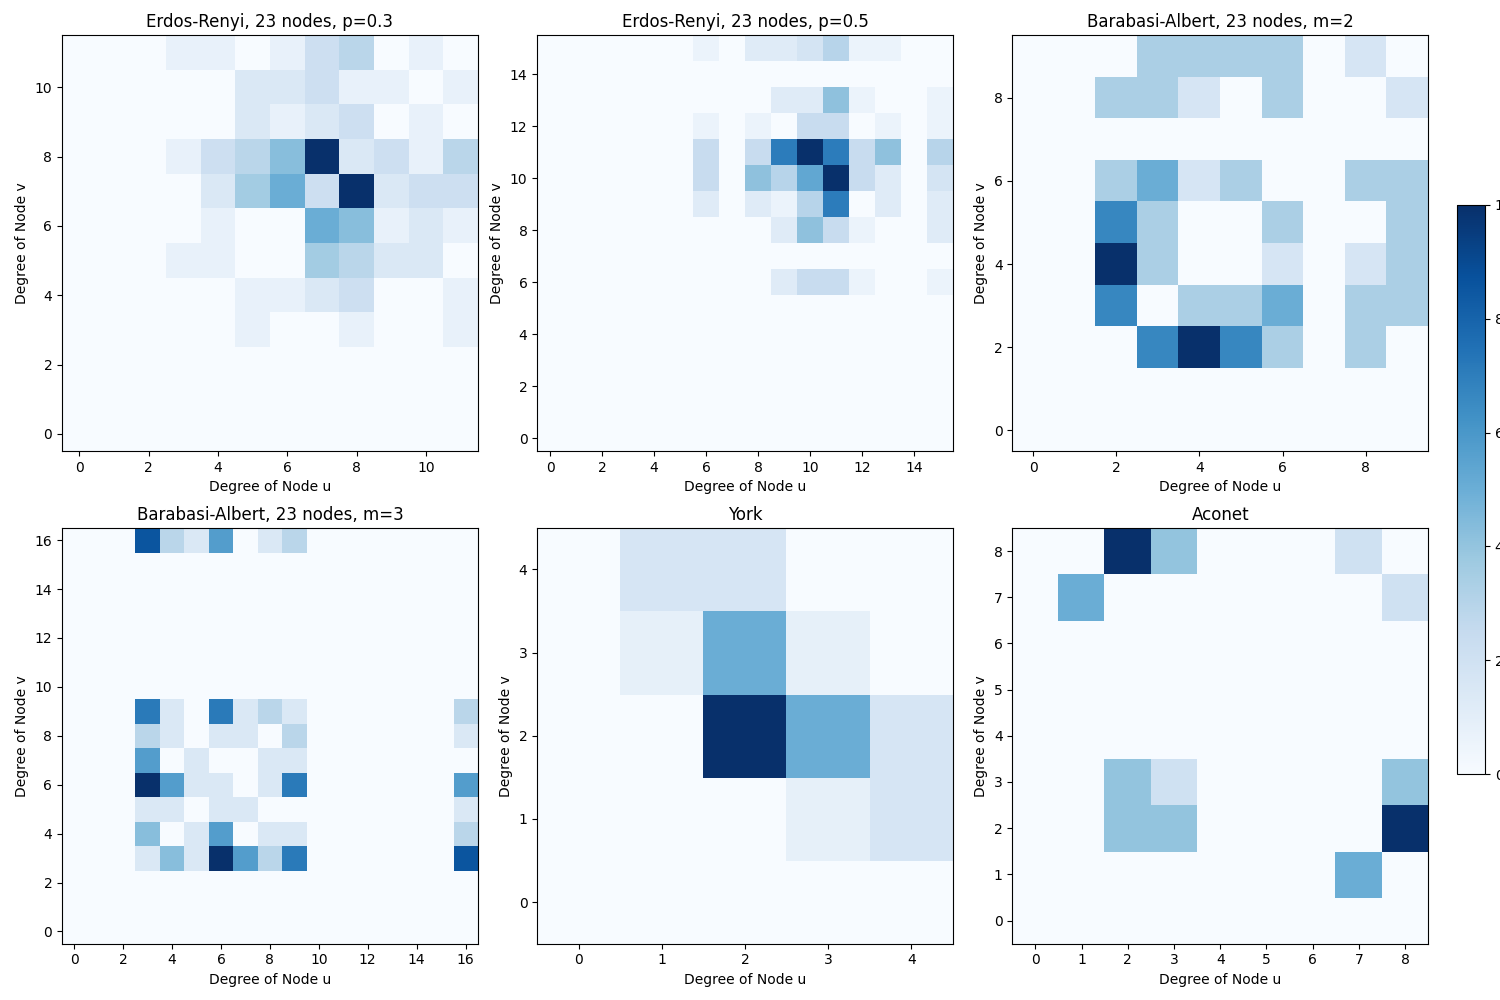
\includegraphics[width=0.9\linewidth]{images/FINAL-TOPO-COMP/Degree-correlation-matrices/23-matrix.png}
    \caption{Degree correlation matrix, set 4}
    \label{fig:enter-label}
\end{figure}
None of the four generated topologies have a similar degree correlation coefficient to the real-world topologies, with values ranging from -0.01 to -0.23 they are weakly assortative networks. However, the similarity is further established between the Erdos-Renyi p=0.3 and Barabasi-Albert m =3 models, both having comparible values of -0.12 and -0.23 respecitvely. Both York and Aconet are more strongly Assoratitive networks, with degree correlation coefficients of -0.51 and -0.4 respectively. 

\begin{figure}
    \centering
    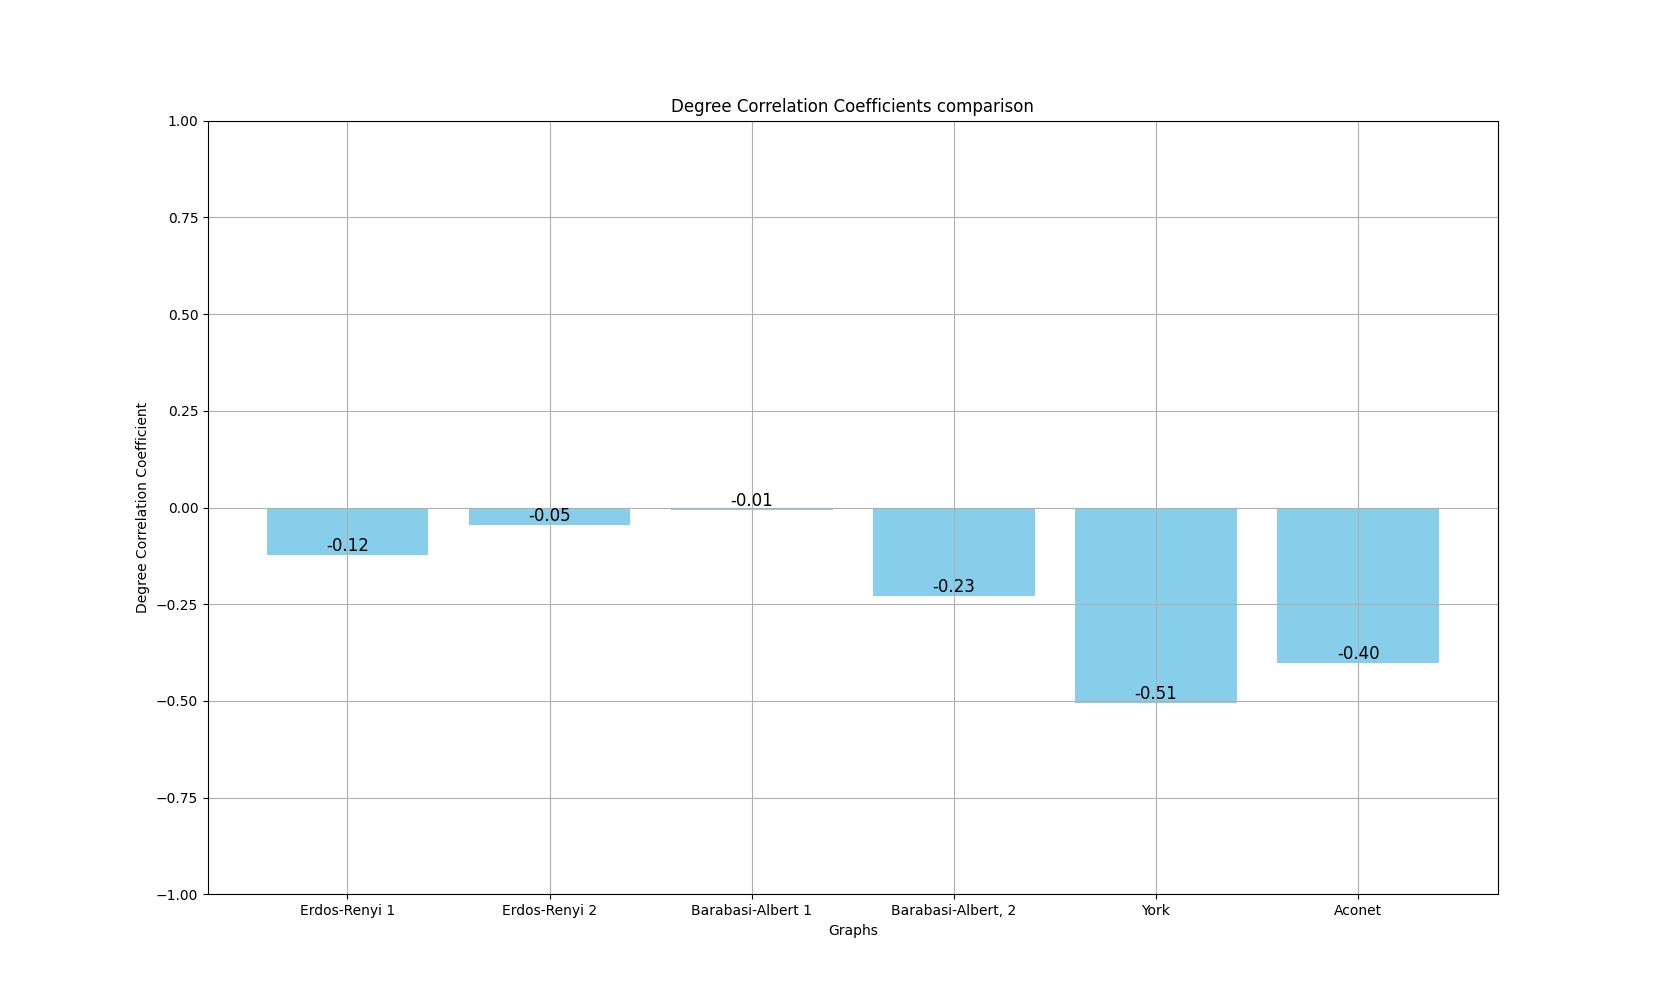
\includegraphics[width=0.9\linewidth]{images/FINAL-TOPO-COMP/Degree-correlation-coeff/deg-coeff-23.png}
    \caption{Degree correlation coefficient, set 4}
    \label{fig:enter-label}
\end{figure}

\subsubsection{Topology set 5}
Much like the previous topology set, the real-world topologies have a relatively flat profile. This might suggest a trend that increasing the network size flattens the shortest path length distribution. Additionally, also much like the previous topology sets the Erdos-Renyi p=0.3 and Barabasi-Albert m=3 topologies have very similar distributions. 
\begin{figure}
    \centering
    distribution 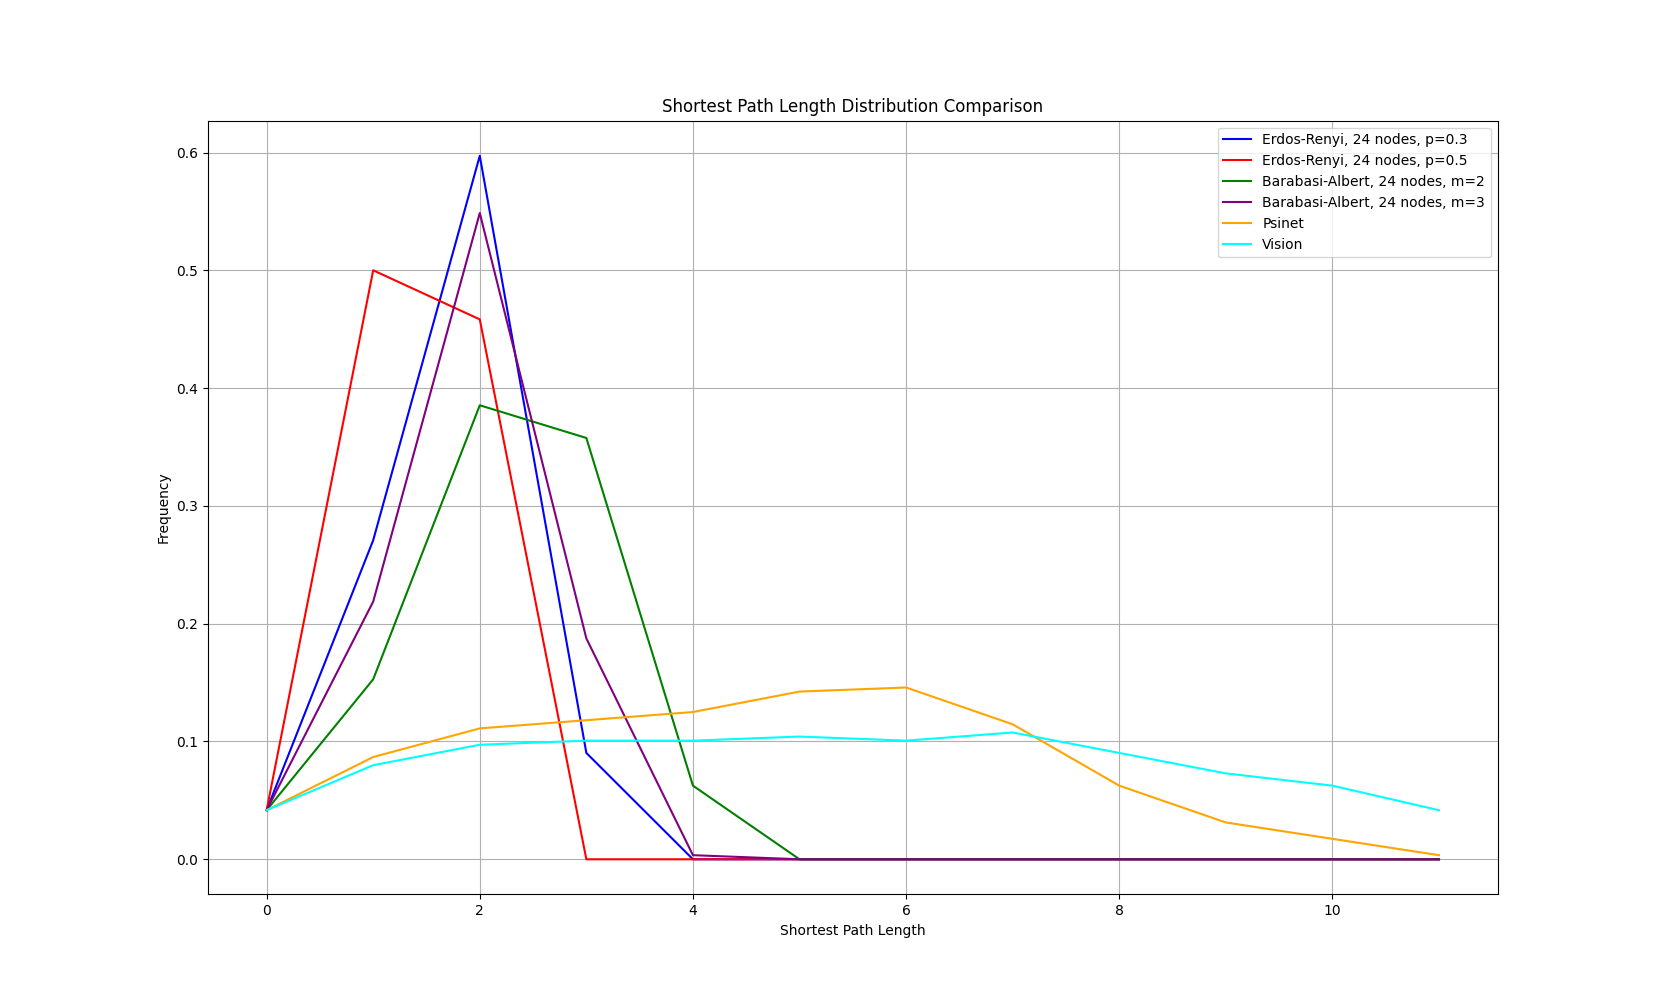
\includegraphics[width=0.9\linewidth]{images/FINAL-TOPO-COMP/line-24.png}
    \caption{Shortest path length distribution comparison, set 5}
    \label{fig:enter-label}
\end{figure}

\begin{figure}
    \centering
    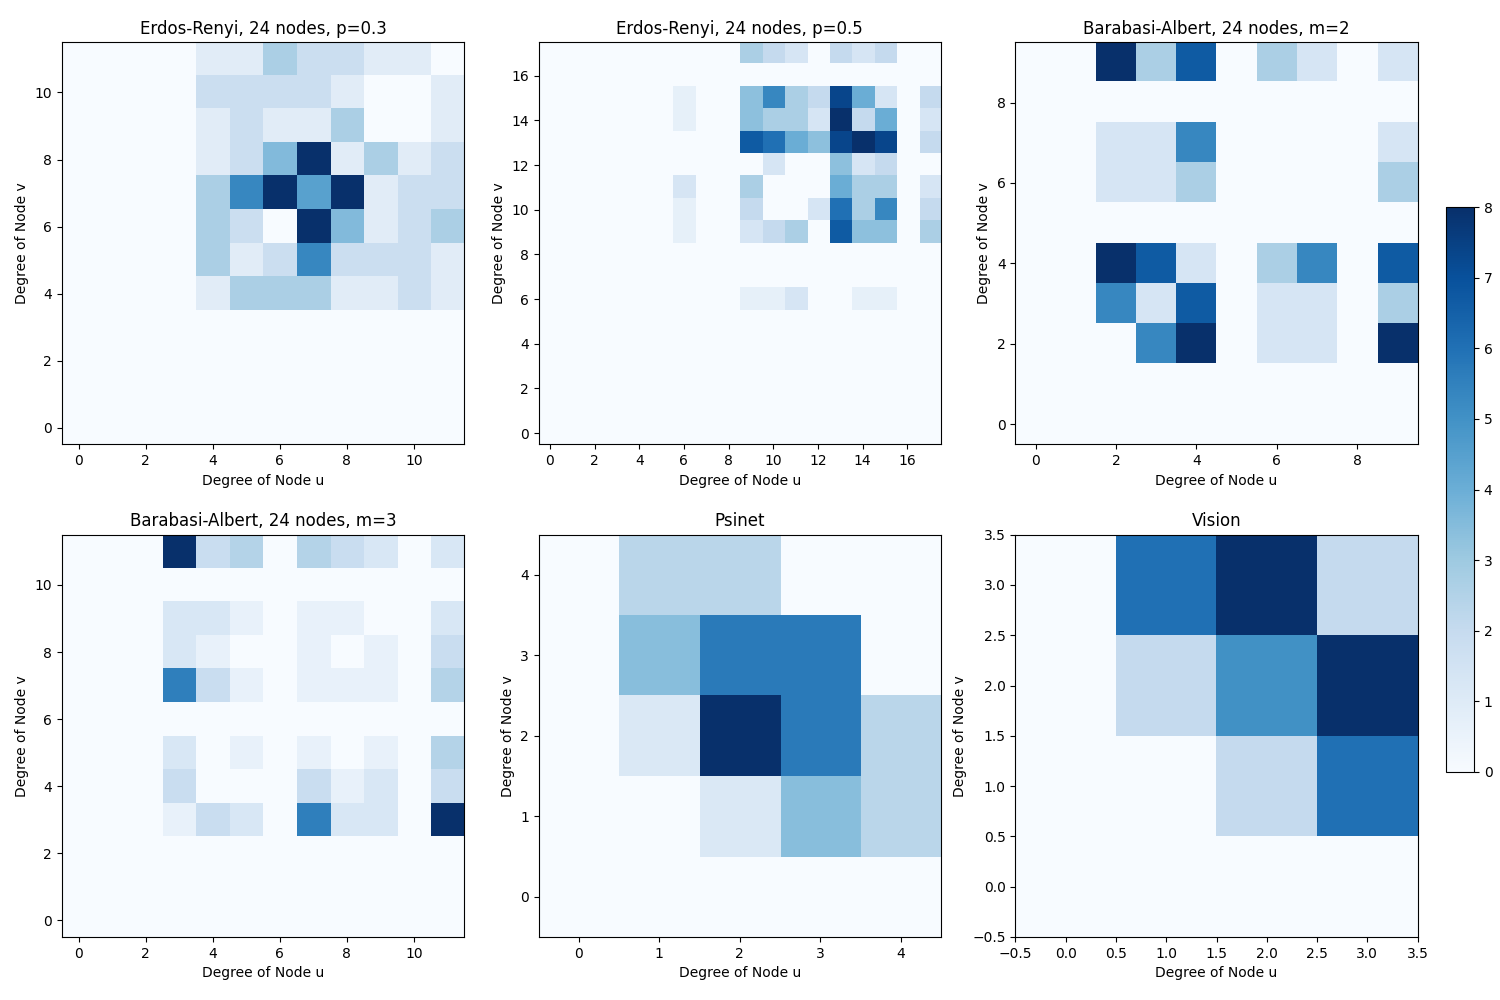
\includegraphics[width=0.9\linewidth]{images/FINAL-TOPO-COMP/Degree-correlation-matrices/24-matrix.png}
    \caption{Degree correlation matrix, set 5}
    \label{fig:enter-label}
\end{figure}

The comparison between the topology set shows an increasing degree correlation coefficient, with both the Erdos-Renyi models having values -0.05 and -0.10 which has some disparity with Psinet and Vision's degree corelation coefficient values of -0.37 and -0.43 respectively. Out of the generated topologies, only the Barabasi-Albert m=3 model is comparable to Psinet and vision, with a degree correlation coefficient of -0.37. 
\begin{figure}
    \centering
    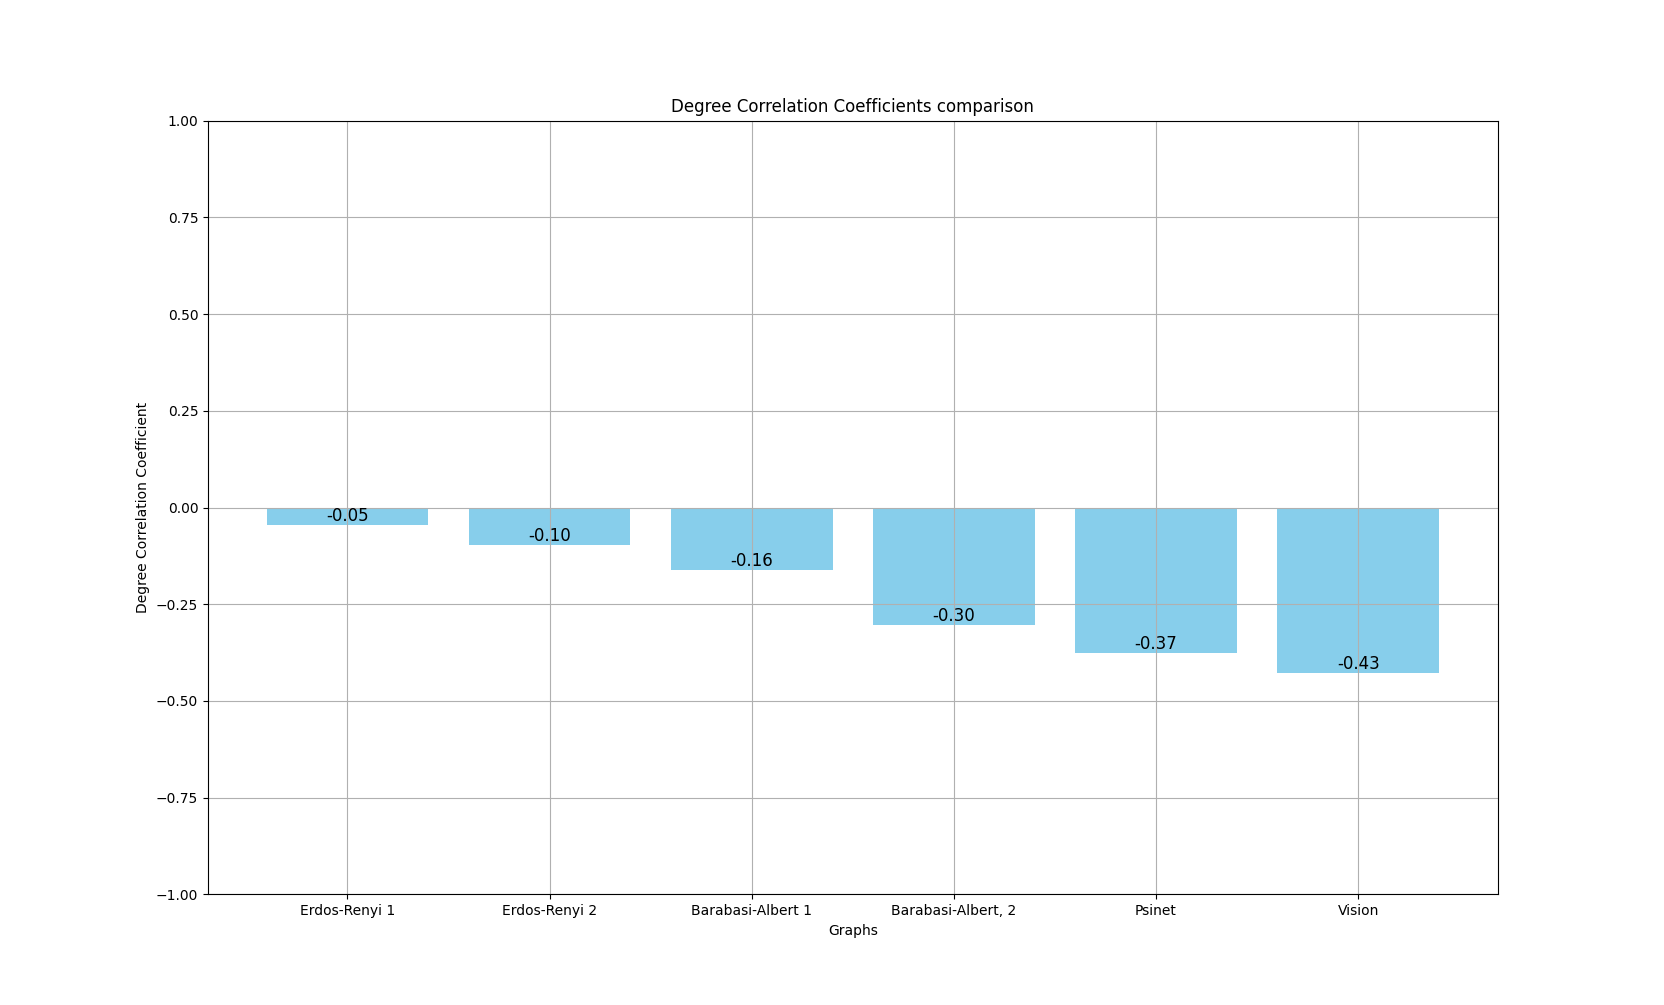
\includegraphics[width=0.9\linewidth]{images/FINAL-TOPO-COMP/Degree-correlation-coeff/deg-coeff-24.png}
    \caption{Degree correlation coefficient, set 5}
    \label{fig:enter-label}
\end{figure}

\subsubsection{Topology set 6}
Both Bbnplanet and Integra have very similar shortest path length distributions and a much flatter profile compared with the generated topologies; much like several of the previous real-world topologies. Furthermore, much like previous topology sets both the Erdos-Renyi p=0.3 model and Barabasi-Albert m=3 model have comparable distributions. 
\begin{figure}
    \centering
    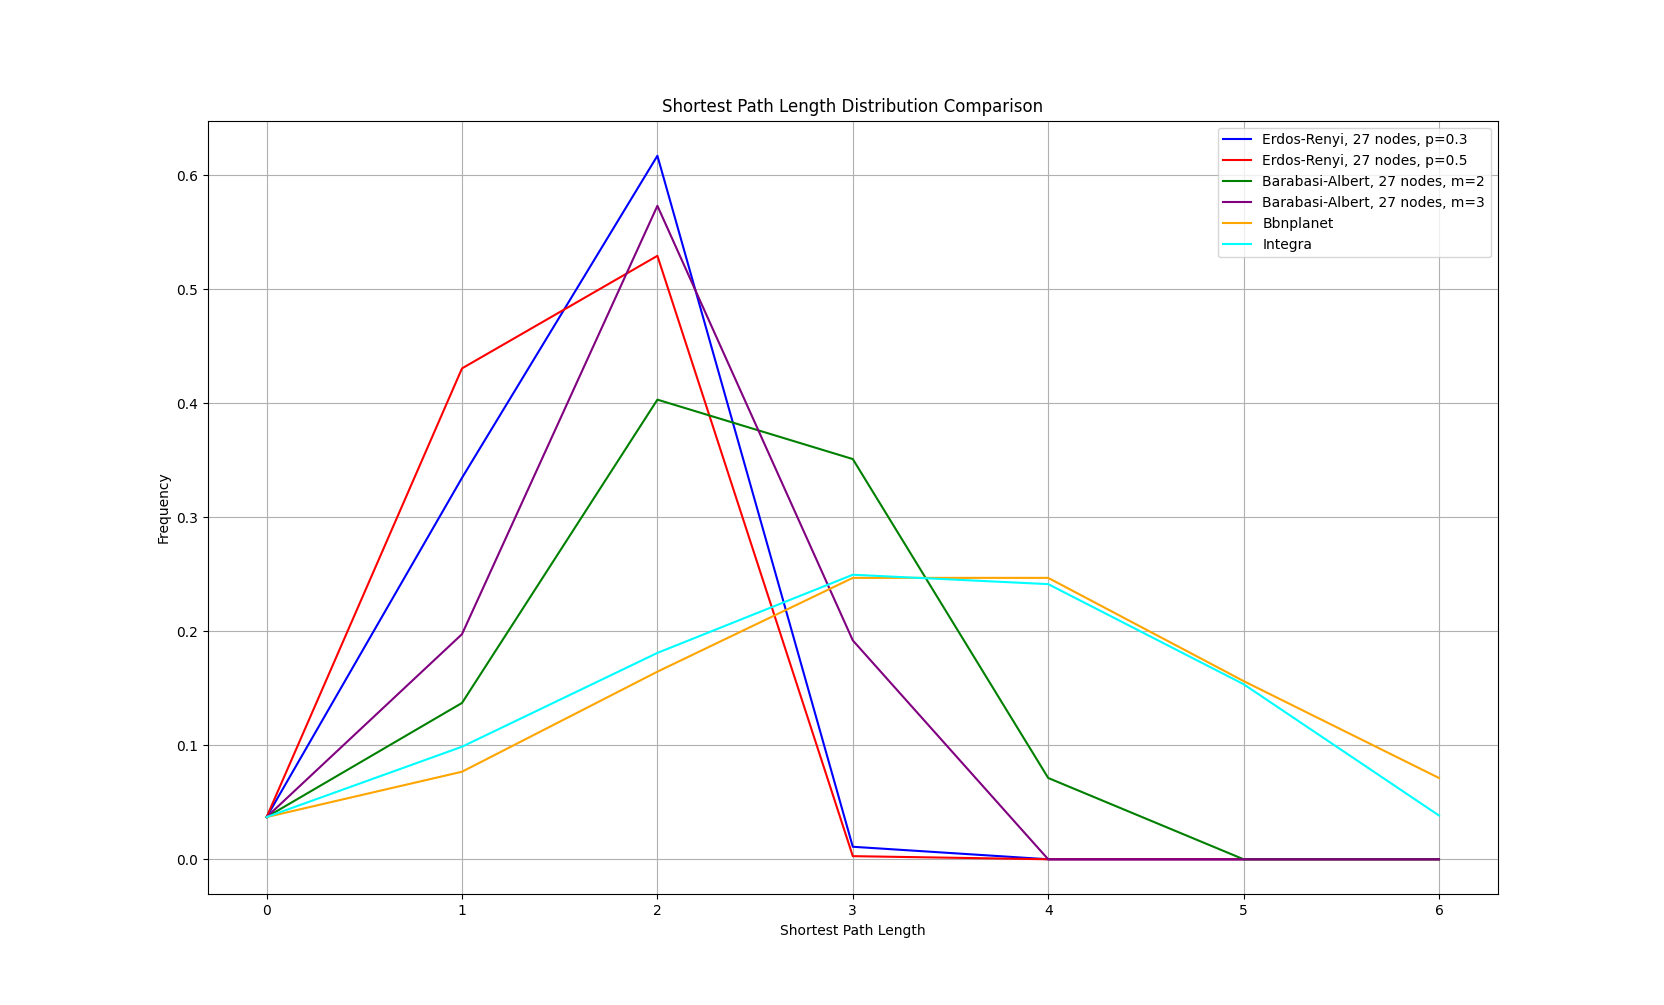
\includegraphics[width=0.9\linewidth]{images/FINAL-TOPO-COMP/line-27.png}
    \caption{Shortest path length distribution comparison, set 6}
    \label{fig:enter-label}
\end{figure}

\begin{figure}
    \centering
    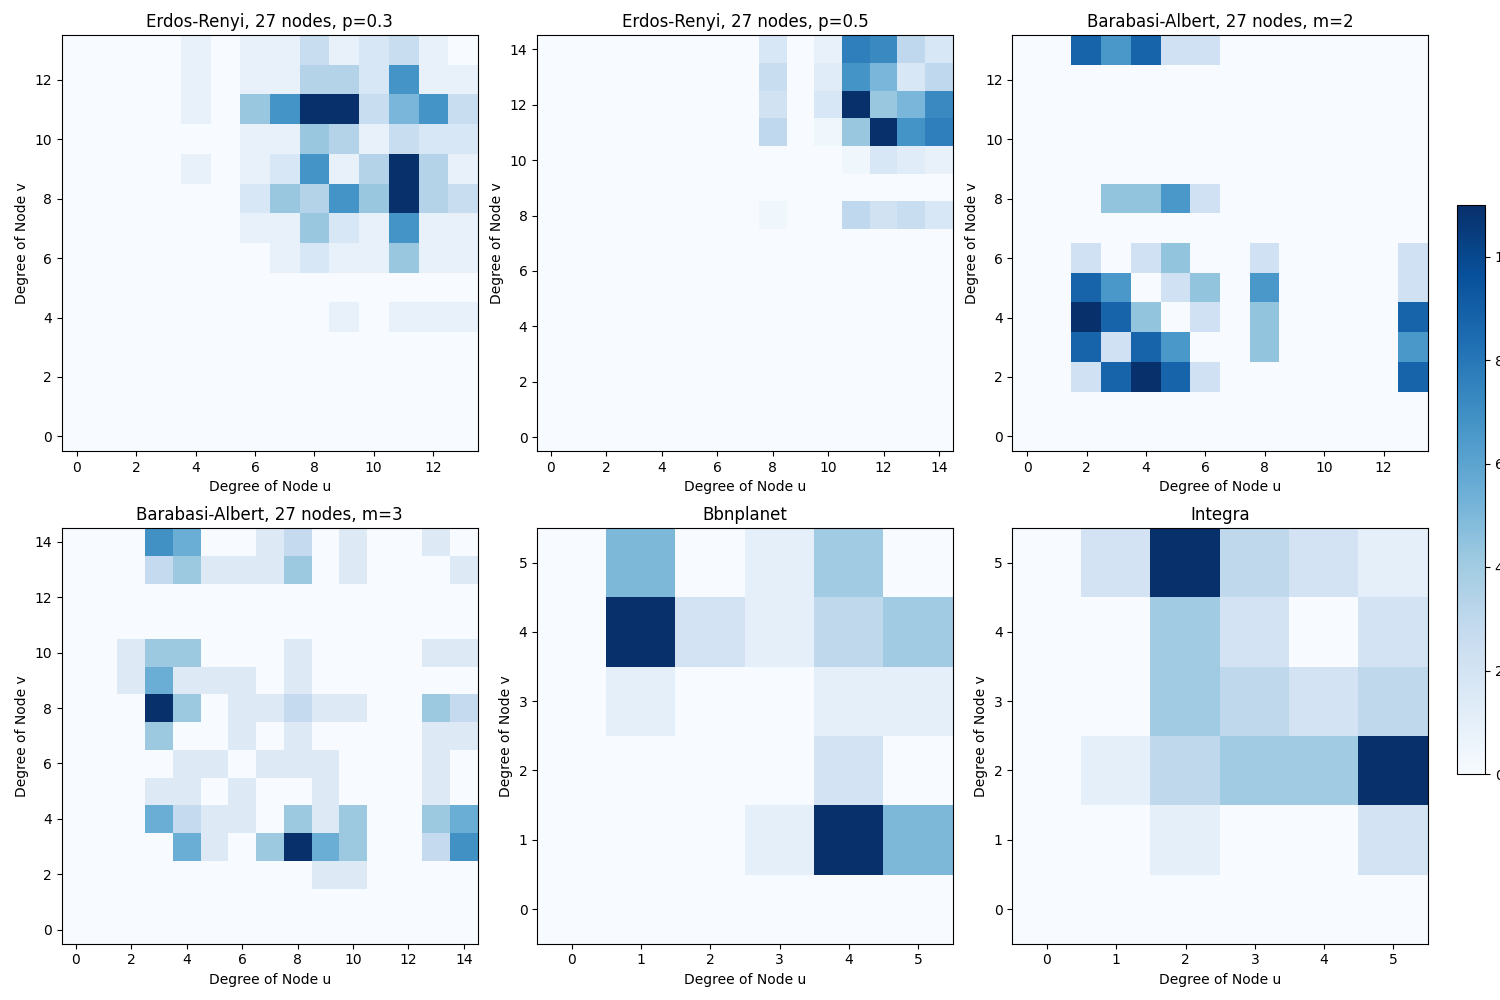
\includegraphics[width=0.9\linewidth]{images/FINAL-TOPO-COMP/Degree-correlation-matrices/27-matrix.png}
    \caption{Degree correlation matrix, set 6}
    \label{fig:enter-label}
\end{figure}

The degree correlation coefficient for both Erdos-Renyi generated topologies are slightly assoratitve, with $r$ values of -0.14 and -0.09 respectively. Additionally, both Barabasi-Albert models have lower degree correlation coefficient relative to the Erdos-Renyi with $r $values of -0.21 and -0.31 respectively. This echos previous results on the prior topology sets, whereby both types of generated models are generally assortative, with the Barabasi-Albert models having an elevated assortativity compared with the Erdos-Renyi models. 

\begin{figure}
    \centering
    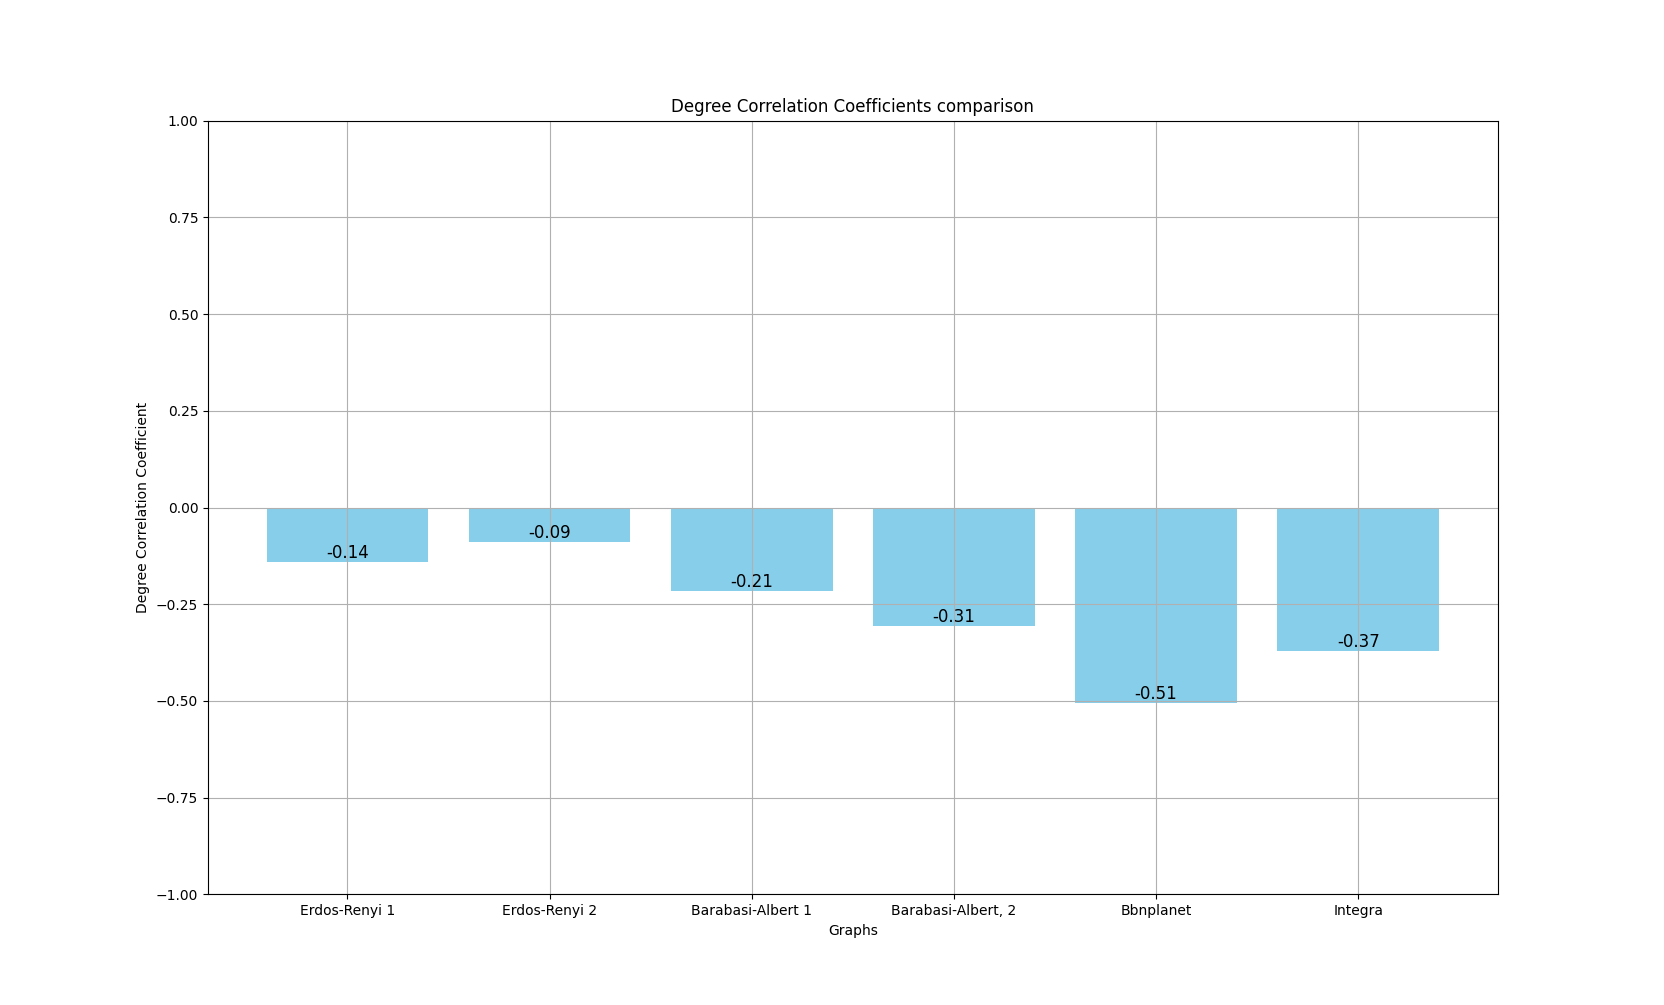
\includegraphics[width=0.9\linewidth]{images/FINAL-TOPO-COMP/Degree-correlation-coeff/deg-coeff-27.png}
    \caption{Degree correlation coefficient, set 6}
    \label{fig:enter-label}
\end{figure}

\subsection{Evaluation}
\subsubsection{Evaluation of Results}
Through evaluation of the comparison using statistical methods between the six sets of generated topologies and real-world topologies, clear trends are revealed. The mean degree correlation coefficient for every topology set was below -0.1, indicating that on average the topologies are assortative. The topology set with size 6 nodes has the lowest mean degree correlation coefficient of approximately -0.4, and the topology set of size 20 nodes has the highest mean degree correlation coefficient of approximately -0.1. The set comprising of topologies of size 13 nodes has the largest distribution.    

\begin{figure}
    \centering
    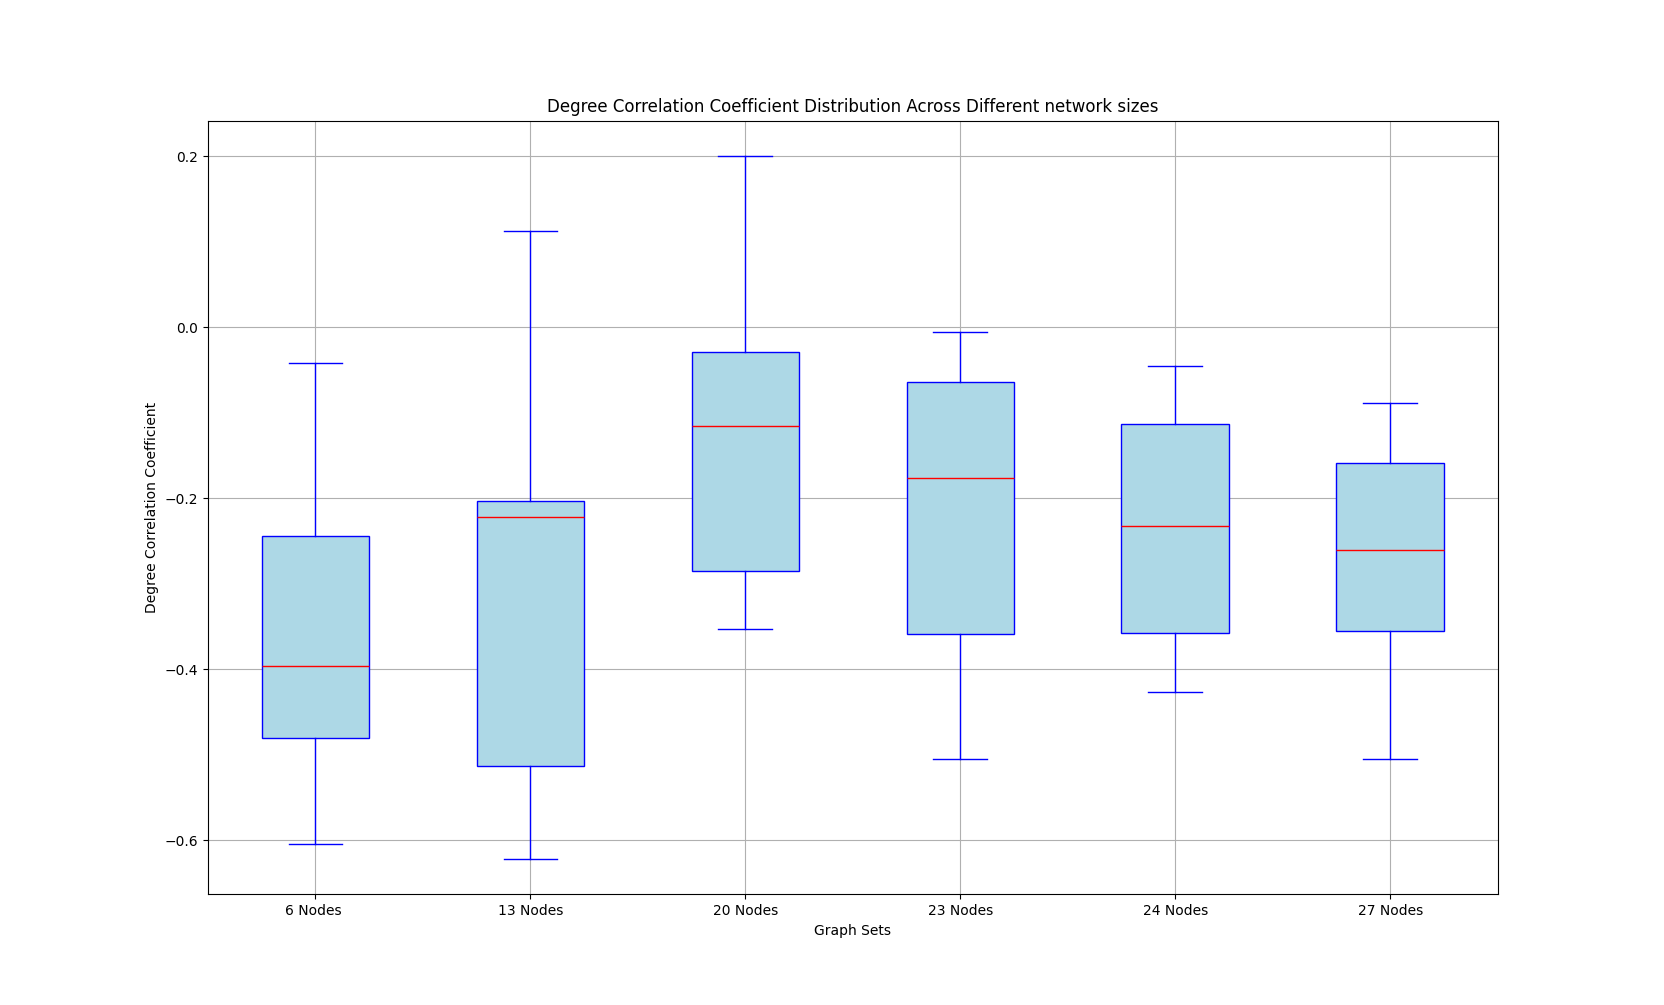
\includegraphics[width=0.9\linewidth]{images/FINAL-TOPO-COMP/Degree-coeff-distrib/Distrib-by-size.png}
    \caption{Degree correlation coefficient distribution across each set}
    \label{fig:enter-label}
\end{figure}

The distribution plot below highlights that there is a distinct difference in degree correlation coefficient between each topology type. This range encompasses the Erdos-Renyi models, which are weakly assortative, the Barabasi-Albert models which are moderately assortative and the real-world models which are the most assortative. This result could be due to the preference in real-world networks to aggregate around central "hubs", which have a high degree and are highly connected. Thus, it can be suggested that this is a characteristic of real-world networks on average, and that if a stochastically generated network is to act as a model for a realistic testing environment it must also have this characteristic. Based on this reasoning, the topologies generated using the Barabasi-Albert model are more representative of real-world networks as their degree corrleation coefficient more closely matches that of real-wold topologies. However, there is also a justification to be made for using topologies generated using the Erdos-Renyi model, as they can provide a diverse and varied experimental environment and increase the available testing space due to their random and un-predictable nature. 

\begin{figure}
    \centering
    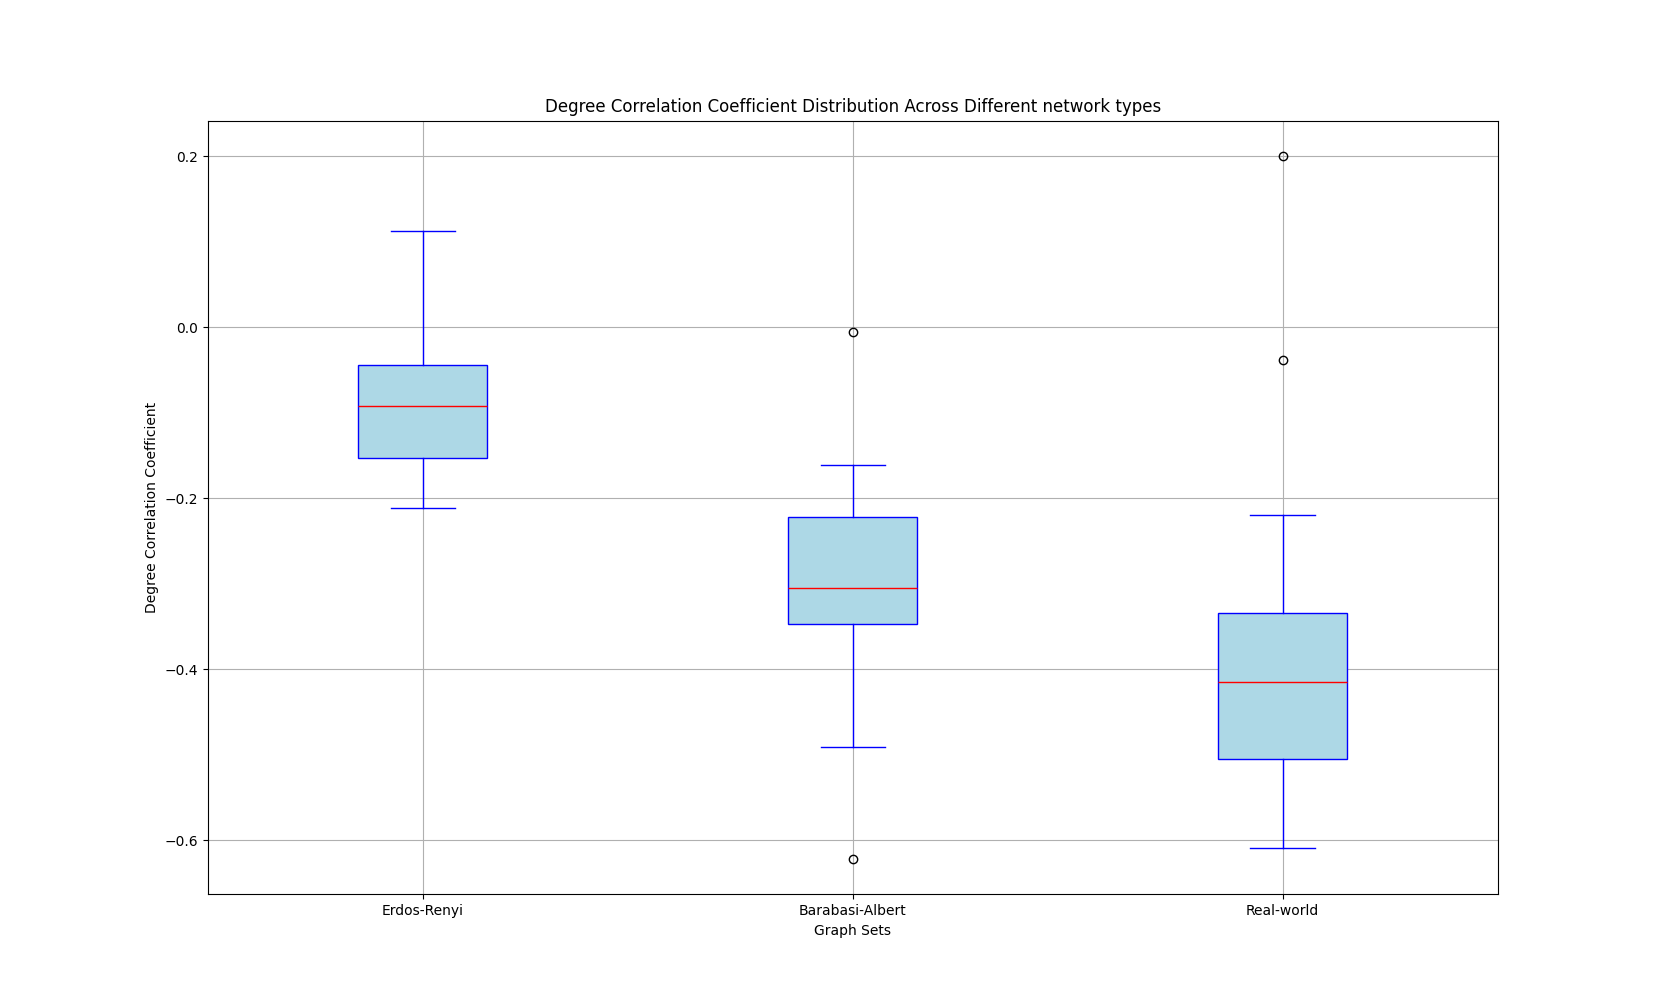
\includegraphics[width=0.9\linewidth]{images/FINAL-TOPO-COMP/Degree-coeff-distrib/Distrib-by-type.png}
    \caption{Degree correlation coefficient distribution across each network topology type}
    \label{fig:enter-label}
\end{figure}

Continuing on from the previous analysis, through plotting the individual degree correlation coefficient distributions the difference between both stochastic models is further highlighted. With the Erdos-Renyi models both being relatively similar, with both having comparable average degree correlation coefficients of approximately -0.1 and relatively similar distributions. The key information which is shown is the difference between both Barabasi-Albert models, with the m=2 model having a much larger distribution and slightly higher average than the m=3 model. This is consistent with the prior comparison with real-world topologies, which the m=3 model was the most closely matched to. 
\begin{figure}
    \centering
    \includegraphics[width=0.9\linewidth]{images/FINAL-TOPO-COMP/Degree-coeff-distrib/Distrib-by-param.png}
    \caption{Degree correlation coefficient distribution of the randomly generated models}
    \label{fig:enter-label}
\end{figure}

The below plot reflects the distribution of a larger set of 28 real-world topologies, with an average degree correlation coefficient of approximately -0.4 this further illustrates the assortative tendency of such networks. There are outliers which have significantly higher degree correlation coefficients above 0, showing some variance between networks, however this is to be expected with a larger set of data encompassing different network sizes. 

\begin{figure}
    \centering
    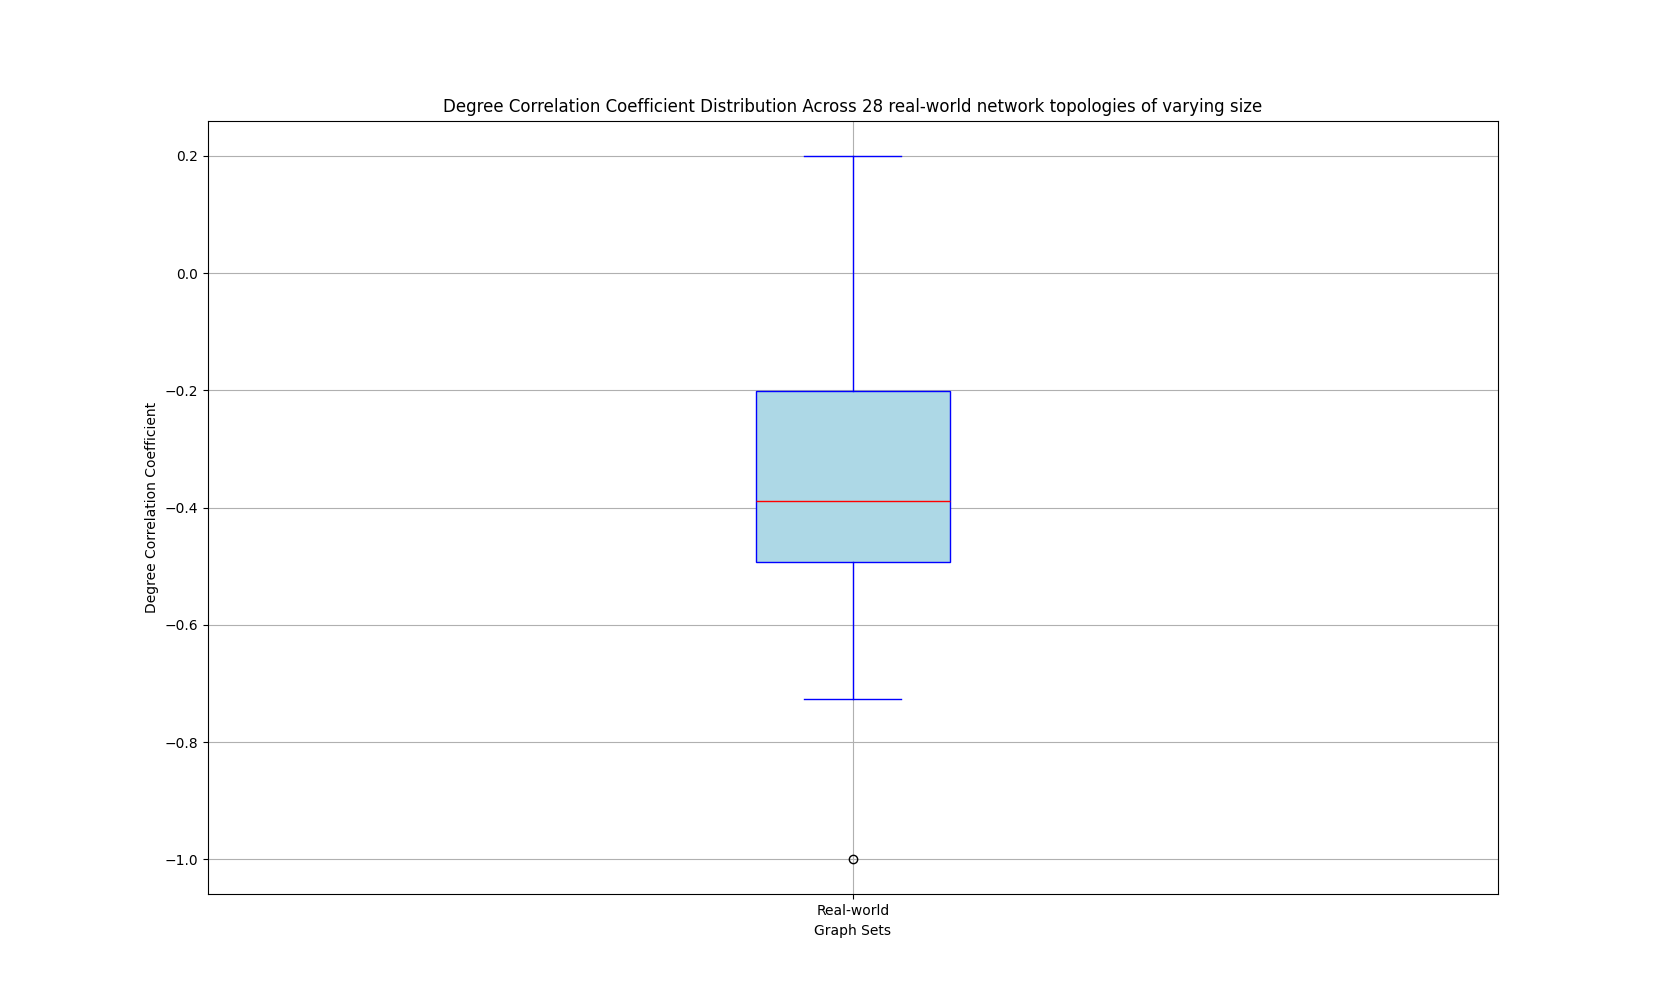
\includegraphics[width=0.9\linewidth]{images/FINAL-TOPO-COMP/Degree-coeff-distrib/Distrib-28-real-world.png}
    \caption{Degree correlation distribution of 28 real-world network topologies}
    \label{fig:enter-label}
\end{figure}

\subsubsection{Evaluation of project}
% Discuss Limitations of evaluation metric
Analysing real-world and randomly generated topologies has utility by both highlighting important characteristics which define these network structures, and also by establishing the similarities and differences between each topology type across a number of different network sizes. Using the data from this measurement can help establish which of the stochastic models is most closely matched to real-world networks across each topology set, and therefore which would be most suitable to be implemented in a virtual lab context. 

However, this approach has several drawbacks; Firstly the real-world topology set is comprised of networks cover a very large geographical area, often providing coverage across countries, continents and the entire world, thus they might not be an accurate representation of more smaller scale but still significant networks, such as an enterprise intranet which could possibly exhibit different linking structures. Furthermore, smaller networks are often desired to be simulated in a virtual lab context as they represent the environment in which varying tools and methods such as traceroute \cite{jacobson1989traceroute} and ping are deployed. Another limitation of this approach is the restricted variance in the parameters for both models used to generate the topologies, through only implementing two variants of each model per set the possible results are bounded which could therefore negatively impact meaningful analysis; with an additional consequence of this is that a possibly sub-optimal model configuration could be proposed. By including more variance in size for real-world network topologies used in the topology sets, or perhaps as a separate set, the possible discrepancies between smaller and larger networks could be addressed. This would allow for more balanced results which more fully encapsulate real-world topologies as a whole. The small number of parameters used in the generation of the Erdos-Renyi and Barabasi-Albert models could be improved by increasing the number of evaluated parameter configurations for both respectively. This would increase the amount and heterogeneity of available data, which a similar improvement to increasing the variance in the real-world topologies. 

% Discuss how in topology generation / simulation that several extra layers of complexity have not been covered in this report, outline how they possibly could be going forward in future. Such as router image, router configuration, linking protocols, load-balancing, NAT's, ip obsucation, VPNs, etc.
Containerlab \cite{containerlab}, which is a suitable environment in which the evaluated topologies could be implemented for the purpose of experimentation has been suggested. Furthermore, a lab generation pipeline has been proposed, with supporting code which can generate a network topology based on a chosen model, then be parsed to a YML file format which can then be deployed through the containerlab \cite{containerlab} framework as a simulated topology, allowing further analysis and experimentation. This also has the intention of increasing the speed and ease with which varying topologies can be implemented.  However, simulation of the evaluated topologies has not been directly demonstrated, and only mathematical analysis of the topology structures has been provided. The lack of practical analysis of how each topology performs when used in a simulated virtual lab to measure tools such as traceroute and ping means that the practical application of such topologies cannot be verified. This is suggested for future work, whereby a set of commonly used network analysis tools could be used in a virtual lab environment to practically gain more insight into how each topology type performs across varying metrics. 

Furthermore, whilst a network topology can represent the overall structure of a network it does not capture the full complexity and layers which are present in such an environment. One such example of a characteristic which has not been covered is configuration of each individual node/routers in the network, which in a real-world scenario can have significant effects of the behaviour of how traffic flows through such networks and as a consequence how the evaluated model would behave. One such example is load-balancing which is commonly employed to ensure even traffic flow in a network, which this can result in in-consistent routing paths of packets in a topology. There are further features which could be considered, such as the routing protocols used between simulated nodes in the networks, a common example being OSPF \cite{OSPF_new}, which is used to manage packets sent across the network. Addressing these limitations is challenging, as it could potentially introduce too many variables and take the focus away from analysis on topology performance. However, as they are present in real-world networks including these features in a controlled manner could add a further dimension to the virtual network lab and ensure that it more closely represents a real-world scenario. These aspects can be successfully captured in ContainerLab \cite{containerlab} . It has the capacity to fully configure the routers and clients in the implemented networks, and also similarly for the routing protocols used. 

% Discuss symmetry between randomly generated networks and real-world networks
% Discuss other random network generation techniques
Whilst this report focused primarily on the Erdos-Renyi and Barabasi-Albert models, a proposed approach in the methodology to generate stochastic topologies, which hasn't been implemented, was using a topology library. Whereby a set of varying topology structures, are combined in random formations to create a composite topology. Each included topology in the set could exhibit differing characteristics ensure amble variance. To ensure that the created networks conform to a structure which is realistic and also add parameters which can control the resultant structure, each topology in the set could have an associated weight $w$, and bias $b$. For example, a more commonly observed topology such as a bus topology could have a higher weight to reflect this. This model could also be refined through defining the addition strategy from which topologies are combined. Similarly to the selection of topologies from the set ,the selection of node which the newest topology is attached to could also be defined as a controllable parameter. Several approaches could be used, such as weighting each node based on their degree; either positively $w>0$ which would likely result in an assortative network, negatively $w<0$ which would likely result in a disassortative network ,or $w=0$ which would likely result in a neutral network. As it was observed in evaluation of the real-world topologies that there is a tendency for such networks to be assortative, if such an approach is to be employed with the intention of emulating realistic structures it to could be suggested to use a positive weighting strategy. Further addition approaches could be used, such as radially weighting each node in the network from the centre, however the utility of such approaches remains unsubstantiated. 


% Expand on proposed Topology library generated structure concept - could be an interesting contribution.

% Discuss other topology modalities, i.e Peer2Peer


%For applications, this will describe the evaluation of the system and how this evaluation answers the research questions. It will describe the evaluation framework, e.g. usability tests, use of external datasets and benchmarks, customer acceptance tests, and the results. 